% !TeX encoding = UTF-8
% !TeX spellcheck = sk_SK
\documentclass[]{tukediphc}
%% -----------------------------------------------------------------
%% tento subor ma kodovanie utf-8
%% 
%% na kompilaciu pouzivajte format pdflatex 
%%
%% V pripade problemov kontaktujte Jána Bušu st. (jan.busa@tuke.sk)
%%
%% November 2015
%% -----------------------------------------------------------------
%%
%\usepackage[dvips]{graphicx}
%\DeclareGraphicsExtensions{.eps}
\usepackage[pdftex]{graphicx}
\usepackage{ragged2e}
\usepackage{pdfpages}


\DeclareGraphicsExtensions{.pdf,.png,.jpg,.mps,.svg}
\graphicspath{{figures/}} % priecinok na obrazky
%%
 

%\usepackage[utf8]{inputenc}  % je v cls-subore
%\usepackage[T1]{fontenc}  % je v cls-subore
\usepackage{lmodern,textcase}
\usepackage[slovak]{babel}
\def\refname{Zoznam použitej literatúry}
\usepackage{latexsym}
\usepackage{dcolumn} % zarovnanie cisiel v tabulke podla des. ciarky
\usepackage{hhline}
\usepackage{amsmath,amsfonts,amssymb}

\usepackage{tikz}
\usetikzlibrary{shapes.geometric, arrows}

\usepackage{indentfirst}
\usepackage{parskip}
\setlength{\parskip}{1em}

\usepackage{nicefrac} % pekne zlomky
\usepackage{upgreek} % napr. $\upmu\mathrm{m}$ pre mikrometer ...
\usepackage[final]{showkeys}%color%notref%notcite%final
\usepackage[slovak,noprefix]{nomencl}
 
\makeglossary % prikaz na vytvorenie suboru .glo



\usepackage{listings}
\usepackage{pythonhighlight}
\lstnewenvironment{mypython}[1][]{\lstset{style=mypython,#1}}{}





% Pouzit v pripade velkeho poctu subsection v tableofcontents
% \makeatletter
% \renewcommand*\l@subsection{\@dottedtocline{2}{1.5em}{3.5em}}
% \newcommand*\l@subsection{\@dottedtocline{2}{1.5em}{2.3em}}
% \newcommand*\l@subsubsection{\@dottedtocline{3}{3.8em}{3.2em}}
% \makeatother


%\def\thefigure{\Roman{section}.\arabic{figure}}

%\usepackage{parskip}% 'zhusti' polozky obsahu
%% Cislovane citovanie
\usepackage[numbers]{natbib}

%%
%% Citovanie podľa mena autora a roku
%\usepackage{natbib} \citestyle{chicago}
% -----------------------------------------------------------------
%% tlač !!!
\usepackage[pdftex,unicode=true,bookmarksnumbered=true,
bookmarksopen=true,pdfmenubar=true,pdfview=Fit,linktocpage=true,
pageanchor=true,bookmarkstype=toc,pdfpagemode=UseOutlines,
pdfstartpage=1]{hyperref}
\hypersetup{%
baseurl={http://www.tuke.sk/sevcovic},
pdfcreator={pdfcsLaTeX},
pdfkeywords={Multi-robot navigation, target tracking, hunt-ing behavior, cooperative collision avoidance},
pdftitle={Využitie prostriedkov internetu vozidiel v navigácii mobilných robotov},
pdfauthor={Bohdan Tanasov},
pdfsubject={Diplomová práca}
} 
%% nehodiace zakomentujte !
\dippraca{Diplomová práca}
%\bakpraca{Bakalárska práca}
%%
\nazov{Využitie prostriedkov internetu vozidiel v navigácii mobilných robotov}
%% ked praca nema 'podnazov' zakomentujte nasledujuci riadok
%% alebo polozku nechajte prazdnu
\podnazov{}
\jazyk{Slovenský}
% anglicky nazov
\title{Simulation of Cooperation for a Multi-Robotic System}
\autor{Bohdan Tanasov}
\veduciprace{doc. Dr. Ing.~Ján~Vaščák}
\konzultanta{ing.~Dušan~Herich}
% \konzultantb{RNDr.~Marián~Čierny, DrSc.}
\titul{Bc}
\univerzita{Technická univerzita v~Košiciach}
\fakulta{Fakulta elektrotechniky a informatiky}
\skratkafakulty{FEI}
\katedra{Katedra umelej inteligencie}
\skratkakatedry{KUI}
\odbor{Informatika}
\specializacia{Inteligentné systémy}
\abstrakt{Cieľom tejto práce bolo vyvinúť automatizovaný systém riadenia pre bezpilotné lietadlo, ktorý využíva zabudovanú kameru na navigáciu a zber údajov. Systém bol implementovaný pomocou programovacieho jazyka Python spolu s balíkom OpenCV pre algoritmy počítačového videnia a značkami ArUco pre merania, NodeJS a React. 
Pomocou systému môžeme manipulovať s viacerými dronmi a so samostatným dronom z webovej stránky a môžeme vidieť údaje dronov a súradnice dronov v priestore pomocou značiek aruco.
Na záver možno konštatovať, že systém úspešne dosiahol svoj cieľ, ktorým je adaptácia autonómneho navigačného systému pre bezpilotné lietadlá v interiéri. Následne spracované súbory údajov boli dostatočne dobre filtrované, aby sa mohli považovať za adekvátne merania. Program by sa mohol v budúcnosti vylepšiť tak, aby podporoval viac príkazov pre skupiny dronov, napr. postaviť kolo alebo iné postavy. Takýto systém sa dá použiť aj pre priemyselné bezpilotné lietadlá, kde sú polohy AR markerov vopred známe.}
\abstrakte{The objective of this work was to develop an automated control system for an unmanned aircraft that uses an embedded camera for navigation and data collection. The system was implemented using the Python programming language along with the OpenCV package for computer vision algorithms and the ArUco tags for measurements, NodeJS and React. 
Using the system, we can manipulate multiple drones and a single drone from a web page and can see the drone data and drone coordinates in space using aruco tags.
In conclusion, the system has successfully achieved its goal of adapting an autonomous navigation system for drones indoors. The subsequently processed datasets were sufficiently well filtered to be considered as adequate measurements. The program could be improved in the future to support more commands for groups of drones, e.g., build a bike or other figures. Such a system could also be used for industrial drones where the positions of the AR markers are known in advance.}
\keywords{UAV, autonomous navigation, AR marker, positioning, measurements}
\klucoveslova{UAV, autonómna navigácia, AR marker, určovanie polohy, merania}

\datumodovzdania{21.~4.~2023}
\datumobhajoby{20.~5.~2023}
\mesto{Košice}
\pocetstran{\pageref{page:posledna}}
\kategoria{Záverečná práca} 

\begin{document}
\renewcommand{\figurename}{Obrázok}	
\renewcommand\theHfigure{\theHsection.\arabic{figure}}
\renewcommand\theHtable{\theHsection.\arabic{table}}

\prvastrana

\titulnastrana 

%\analytickylist


%\errata % zaciatok erraty
%Ak je potrebné, autor na tomto mieste opraví chyby, ktoré našiel po
%vytlačení práce. Opravy sa uvádzajú takým písmom, akým je napísaná
%práca. Ak zistíme chyby až po vytlačení a zviazaní práce, napíšem
%erráta na samostatný lístok, ktorý vložíme na toto miesto. Najlepšie je
%lístok prilepiť \citep{kat}.
%
%Forma:
%
%%\tabcolsep=10pt
%\begin{table}[!hb]
%	\centering
%	\begin{tabular}{|c|c|c|c|}\hline
%Strana & Riadok & Chybne & Správne \\\hline\hline
%12 & 6 & publikácia & prezentácia \\\hline
%22 & 23 & internet & intranet \\ \hline
%& & & \\\hline
%& & & \\\hline
%	\end{tabular}
%\end{table}
%\kerrata % koniec erraty

\abstraktsk % abstrakt v SK 

\abstrakteng % abstrakt v ENG

\kabstrakt % koniec abstraktov, nova strana

% Na tomto mieste bude vložené zadanie diplomovej práce
% \zadanieprace{}
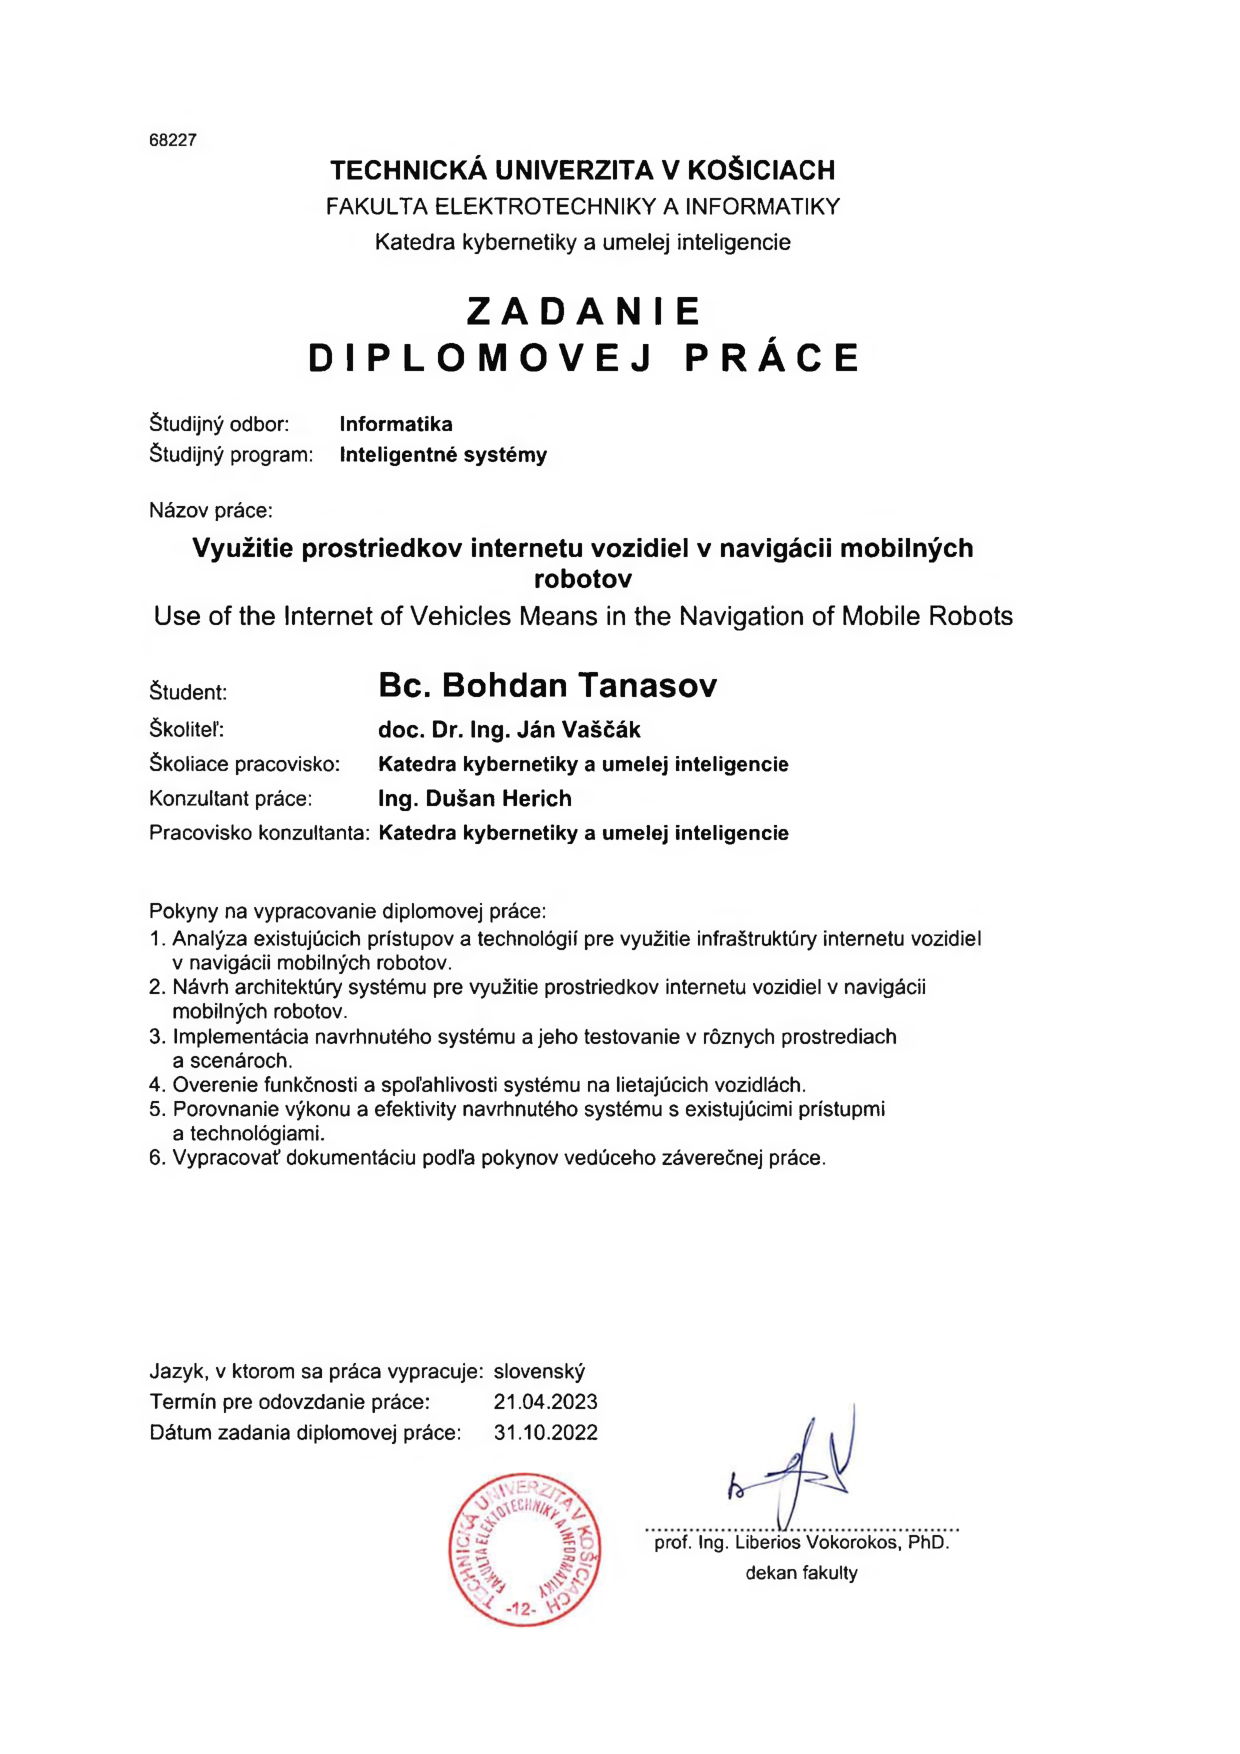
\includepdf[pages=-]{zadavaci-list.pdf}

\cestnevyhlasenie
% Niektorí autori metodických príručiek o~záverečných prácach sa
% nazdávajú, že takéto vyhlásenie je zbytočné, nakoľko povinnosť
% vypracovať záverečnú prácu samostatne, vyplýva študentovi zo zákona a
% na autora práce sa vzťahuje autorský zákon.

\podakovanie
Najskôr by som sa chcel poďakovať vedúcemu bakalárskej práce doc. Dr. Ing. Jánovi Vaščakovi. Príležitosť komunikovať s docentom Vaščakom bola vždy otvorená, kedykoľvek som narazil na problémové miesto alebo mal otázku o svojom výskume alebo písaní. Dôsledne pripúšťal, aby tato práca bola mojou vlastnou, ale vždy, keď si myslel, že to potrebujem, ma nasmeroval správnym smerom.

Na záver musím svojim rodičom poďakovať za to, že mi počas rokov štúdia a pri výskume a písaní tejto práce poskytovali neutíchajúcu podporu a neustále povzbudzovanie. Bez nich by tento úspech nebol možný. Ďakujem.
\kpodakovania

\predhovor
Téma práce sa zaoberá využitím dronov Tello v skupinovej koordinovanej misii, kde bola navrhnutá a implementovaná webová aplikácia, ktorá umožňuje ovládanie viacerých dronov naraz. V práci je tiež popísaná implementácia systému, ktorý umožňuje sledovanie pozície dronov pomocou kamery a detekcie Aruco markerov.
Cieľom tejto práce bolo ukázať, ako efektívne ovládať viacero dronov naraz pomocou jednoduchej webovej aplikácie a koordinovaného systému detekcie pozície dronov. V práci sa tiež zaoberáme riešeniami problémov pri použití viacerých dronov naraz a analyzujeme výsledky našich experimentov a testov.
% Zvýšil sa záujem o výskum v systémoch zložených z viacerých autonómnych mobilných robotov vykazujúcich kooperatívne správanie. Konštruujú sa skupiny mobilných robotov s cieľom študovať také problémy, ako je skupinová architektúra, konflikt zdrojov, pôvod spolupráce, učenie sa a geometrické problémy. Doposiaľ bolo opísaných málo aplikácií kooperatívnej robotiky a teória podpory je stále v štádiu formovania. V tejto prace bol vytvorený multi-robotický projekt a diskutované problémy a variácie ich riešenia 
\kpredhovoru

\thispagestyle{empty}
\tableofcontents
\thispagestyle{empty}

\newpage

\thispagestyle{empty}

{	\makeatletter
	\renewcommand{\l@figure}{\@dottedtocline{1}{1.5em}{3.5em}}
	\makeatother
	\listoffigures}

%\addcontentsline{toc}{section}{\numberline{}Zoznam obrázkov}
%\listoffigures


\newpage

\thispagestyle{empty}
%\addcontentsline{toc}{section}{\numberline{}Zoznam tabuliek}
\listoftables

\thispagestyle{empty}
\newpage
 
\thispagestyle{empty}
%\addcontentsline{toc}{section}{\numberline{}Zoznam symbolov a
%skratiek}
\printglossary % vlozenie zoznamu skratiek a symbolov
\newpage

%\addcontentsline{toc}{section}{\numberline{}Slovník termínov}
\slovnikterminov

\begin{description}
	\item[Webová aplikácia] - softvérová aplikácia typu klient-server, v ktorej klient (alebo používateľské rozhranie) beží vo webovom prehliadači.
	\item[Node.js] - open-source, multiplatformné, back-endové prostredie pre beh JavaScriptu, ktoré beží na engine V8 a vykonáva kód JavaScriptu mimo webového prehliadača.	
	\item[BE server] - backendový server, ktorý spravuje údaje a logiku aplikácie a spracováva požiadavky z front-endu.	
	\item[Tinkerboard] - jednodoskový počítač malých rozmerov určený pre počítačových nadšencov a domácich majstrov.	
	\item[ArUco markery] - typ fiduciálnych značiek, ktoré možno použiť v aplikáciách rozšírenej reality.	
	\item[Program pre drony] - softvér, ktorý beží na palubnom počítači dronu a ovláda jeho pohyby a senzory.
	\item[Detekcia markera] - proces detekcie a identifikácie markera na obrázku alebo videu.	
	\item[Výpočet polohy] - proces určovania polohy objektu vzhľadom na známy referenčný bod alebo objekt.	
	\item[Absolútne súradnice] - presná poloha objektu v priestore, zvyčajne vyjadrená v súradniciach X, Y a Z.	
	\item[Režim viacerých dronov] - režim, v ktorom sa súčasne ovláda viacero dronov.	
	\item[Režim jedného dronu] - režim, v ktorom sa súčasne ovláda len jeden dron.	
	\item[Informácie o stave dronu] - informácie o aktuálnom stave dronu vrátane jeho polohy, nadmorskej výšky, úrovne nabitia batérie atď.
	\item[Jedinečné ID] - jedinečný identifikátor pridelený každému dronu na odlíšenie od ostatných.
\end{description}

\kslovnikterminov
%
% !TeX encoding = UTF-8
% !TeX spellcheck = sk_SK
% !TeX root=tukedip.tex

\section*{Úvod}
\addcontentsline{toc}{section}{\numberline{}Úvod}
\setcounter{page}{1}
Drony sa v posledných rokoch stávajú čoraz populárnejšími vďaka svojej schopnosti vykonávať širokú škálu úloh, ktoré by inak boli pre človeka náročné alebo nebezpečné. Schopnosť ovládať viacero dronov súčasne otvára ešte viac možností ich využitia. Na dosiahnutie tohto cieľa je potrebné vyvinúť riadiaci systém, ktorý umožní efektívne a intuitívne ovládanie viacerých dronov. Cieľom tejto práce je vyvinúť takýto systém pomocou webovej aplikácie React a socketov.

Navrhovaný riadiaci systém umožní používateľovi ovládať viacero dronov Tello súčasne pomocou webového rozhrania. Použitie značiek Aruco umožní dronom zistiť ich polohu a podľa nej sa navigovať, čo umožní ovládať drony v individuálnom aj skupinovom režime. Systém bude pozostávať z backendu Node.js, ktorý bude zabezpečovať komunikáciu medzi webovou aplikáciou a dronmi, ako aj z programu Python bežiaceho na doske Asus TinkerBoard pripojenej ku každému dronu. Každý dron bude mať špecifické ID, čo umožní ich rozlíšenie.

Vývoj takéhoto riadiaceho systému predstavuje niekoľko výziev vrátane potreby zvládnuť komunikáciu v reálnom čase medzi dronmi a webovou aplikáciou, potreby presne zistiť polohu dronov a potreby zabezpečiť, aby sa systém ľahko používal a poskytoval dobrý používateľský zážitok.

Navrhovaný systém má potenciál na využitie v rôznych aplikáciách, ako je napríklad sledovanie pomocou dronov, letecké fotografovanie alebo pátracie a záchranné operácie. Tým, že systém umožňuje efektívne a intuitívne ovládanie viacerých dronov, by mohol pomôcť zvýšiť bezpečnosť a efektívnosť týchto operácií.

Zvyšok tejto práce je usporiadaný takto. V časti 2 sa uvádza prehľad príslušných technológií a metód, ktoré boli použité pri vývoji systému. V časti 3 je opísaný proces vývoja riadiaceho systému vrátane krokov vykonaných pri návrhu, implementácii a testovaní systému. V časti 4 sú uvedené výsledky práce vrátane podrobného opisu vyvinutého systému, jeho vlastností, používateľského rozhrania a funkčnosti, ako aj ukážky možností systému prostredníctvom príkladov použitia. V časti 5 sa hodnotí výkonnosť a použiteľnosť systému pomocou príslušných metrík a spätnej väzby od používateľov. Nakoniec sa v oddiele 6 uvádza zhrnutie výskumnej otázky, cieľov a prínosov, ako aj diskusia o obmedzeniach systému a možných cestách pre budúcu prácu a zlepšenie.
%
% !TeX encoding = UTF-8
% !TeX spellcheck = sk_SK
% !TeX root=tukedip.tex
\section{Formulácia úlohy}
\textbf{Spracovať prehľad metód kooperácie v rámci multi-robotických aplikácií.} Táto časť bakalárskej práce obsahuje popis úloh, ktoré sa riešia pri vzájomnej interakcii viacerých robotov. 
Táto kapitola obsahuje prehľad robotov, kontrolné metódy, komunikačné metódy a problémy, ktoré sa vyskytujú pri vývoji algoritmov pre multi-robotický systém.\newline\newline
% \bigskip
\textbf{Výber vhodnej metódy robotickej kooperácie a návrh jej realizácie.} Táto časť popisuje proces výberu najvhodnejšej metódy na implementáciu 
multi-robotického projektu na základe výhod a nevýhod rôznych metód uvedených v predchádzajúcej časti.\newline\newline
% \bigskip
\textbf{Softvérovo navrhnúť systém pre kooperáciu robotov. } Táto časť bude obsahovať prehľad softvéru potrebného na vypracovanie bakalárskeho projektu a tiež popis metód a prístupov použitých pri práci na projekte.\newline\newline
% \bigskip
\textbf{Vykonať simulačné experimenty a ich vyhodnotiť. } Táto kapitola predstavuje výsledky a vyhodnotenie simulačných experimentov vykonaných pre rôzne situácie. Každá simulácia má svoj vlastný popis a ku každej je pridaný záver\newline\newline
% \bigskip
\textbf{Vypracovať dokumentáciu podľa pokynov vedúceho záverečnej práce.} Posledný bod bude súvisieť s prípravou dokumentácie a popisom celého procesu vývoja tohto projektu. 

%
% !TeX root=tukedip.tex
% !TeX encoding = UTF-8
% !TeX spellcheck = sk_SK
\section{Metódy riadenia v multi-robotických systémoch}
V organizácii a správe systémov s niekoľkými mobilnými robotmi v súčasnosti existuje veľa rôznych prístupov. Nedá sa povedať, že existujú správne alebo nesprávne prístupy, každý zo systémov má svoje výhody aj nevýhody. Rozhodnutie o použití systému sa prijíma na základe konkrétnej úlohy projektu.
V tejto časti sa pozrieme na rôzne metódy riadenia a organizácie multi-robotických systémov, ako aj na ich výhody a nevýhody.

\subsection{Multi-robotické systémy}

Systémy viacerých robotov sú dobré z mnohých ďalších dôvodov. Podľa Aparicio a Lima \citep{aparicio} systémy s viacerými robotmi  ponúkajú robustnosť a prispôsobivosť, aké sa v systémoch s jedným robotom nenachádzajú. Ak je jeden agent v systéme poškodený alebo nefunguje správne, je možné úlohu dokončiť so zvyšnými agentmi. Túto myšlienku možno uplatniť aj pri údržbe. Agenti môžu byť obsluhovaní po jednom, čo vedie k skutočnosti, že systém nie je nečinný, ak sú ostatní roboti schopní pokračovať v plnení úlohy bez prítomnosti ich partnera. Viaceré roboty navyše dokážu pokryť veľkú oblasť a môžu sa špecializovať na menšie úlohy, ktoré postupujú k splneniu väčšej úlohy \citep{aparicio}. Preto je pravdepodobnejšie, že systémy s viacerými robotmi budú spoľahlivo vykonávať veľké a zložité úlohy. Napriek mnohým výhodám systémov viacerých robotov je potrebné vyriešiť niekoľko nevýhod. Najskôr je komunikácia medzi agentmi v systéme výpočtovo zložitá. Podľa Coesa, Nurbakhsh a Sikar %\citep{koes} 
, keď sa systémy s viacerými robotmi rozhodnú, musia brať do úvahy čas potrebný na cestu na konkrétne miesto, čas čakania na príchod ďalších robotov a čas na dokončenie úlohy. V dôsledku toho sú riadiace algoritmy veľmi zložité, pretože systém sa implementuje ťažšie, ak na konkrétnom probléme pracuje viac agentov. Rádiová komunikácia dodáva systému ďalšiu vrstvu zložitosti, pretože si vyžaduje použitie prenosových obvodov a komunikačných protokolov. Preto, aj keď môže byť systém s viacerými robotmi efektívnejší, tento však vyžaduje väčšiu zložitosť než systém s jedným robotom. 

\subsection{Praktické využitie multi-robotických systémov}

Počas výskumu boli objavené aplikácie, ktoré priamo súvisia s mojím projektom. V jednom konkrétnom príklade boli na
premiestnenie nábytku na konkrétne miesta použité dva veľké roboty. V praktickejšom príklade je možné použiť roboty na
presun ťažkých materiálov na stavenisku. Je pravdepodobné, že roboty s takouto úlohou veľmi pomôžu a môžu zvýšiť
efektivitu, ale roboty sú zvyčajne príliš drahé na to, aby boli finančné prospešné.
\vspace{3mm}

\justifying
\noindent 
Jednou z možností v súčasnosti je použitie koordinovaných robotov na skúmanie oblastí, ktoré by mohli byť pre
človeka nebezpečné. Tieto roboty môžu autonómne zvyšovať bezpečnosť alebo vytvárať nebezpečné oblasti. Napríklad oblasť
plná mín môže byť vhodná pre robotov vybavených senzormi určenými na detekciu mín. Potom, čo v mínovom poli, bude robot schopný rozpoznať mínu bez účasti ľudí. nájdení bane môže robot oznámiť polohu míny ďalším robotom.
Ostatní roboti pomocou koordinačných algoritmov a pozičných senzorov budú môcť k míne pristúpiť a pomôcť ju rozobrať
alebo označiť. Roboti sa môžu navzájom rozprávať alebo môžu používať hlavného robota, ktorý dáva každému z nich smer
\citep{mclurkin}. Projekt, ktorý je rovnako jednoduchý ako koordinované tlačenie škatúľ robotom, slúži ako východiskový bod pre
zložitejší a užitočnejší systém, ako sú napríklad robotické vyhľadávače mín.

\subsection{Ovládanie multi-robotických systémov}
Ovládanie systému s viacerými robotmi je vo všeobecnosti náročným problémom. K tejto otázke existujú dva prístupy:
centralizovane riadenie a decentralizovane riadenie \citep{kexu}.

\subsubsection{Centralizovaný systém}
V centralizovanom systéme s niekoľkými robotmi sa ukladajú globálne informácie o stave celého systému. Systém
zhromažďuje informácie o všetkých robotoch a sleduje ich polohu v prostredí. Na základe informácií získaných od robotov
dokáže zostaviť mapu. Tento systém je buď na stacionárnom hostiteľovi, alebo v jednom robote, ktorý zjavne funguje ako
hlavný. Potom majster zorganizuje tím robotov, aby dosiahli spoločný cieľ a naplánuje úlohy pre jednotlivých členov tímu
a dohliada na celý proces.
Táto architektúra sa dá ľahko navrhnúť, ale nie je odolná voči výpadkom komunikácie a nepredvídateľným situáciám.
Centralizované riadenie je zvyčajne vhodné pre obmedzený počet robotov, ktorí pracujú v známom a nemennom prostredí.

\subsubsection{Decentralizovaný systém}
Naproti tomu decentralizované systémy nezahŕňajú žiadneho riaditeľa, ktorý má úplné informácie o stave systému a riadi
celý proces. Naopak, každý robot je autonómna jednotka, ktorá koná v súlade so stavom svojho prostredia. Robot si je
samozrejme vedomý prítomnosti ďalších robotov a môže s nimi komunikovať na miestnej úrovni. Komplexné skupinové
správanie vyplýva z interakcií medzi robotmi a prostredím. Táto architektúra je veľmi robustná, môže dobre fungovať v
nepriateľskom prostredí a je škálovateľná, potenciálne obrovské množstvo homogénnych robotov môžu spolupracovať na
dosiahnutí spoločného cieľa.

\subsection{Problématika riadenia}
Problém s riadením v navigácii mobilných robotov sa rieši dvoma spôsobmi: deliberatívnym a reaktívnym riadením (Obrázok 2 –
1).

\begin{figure}[ht!]
    \centering
    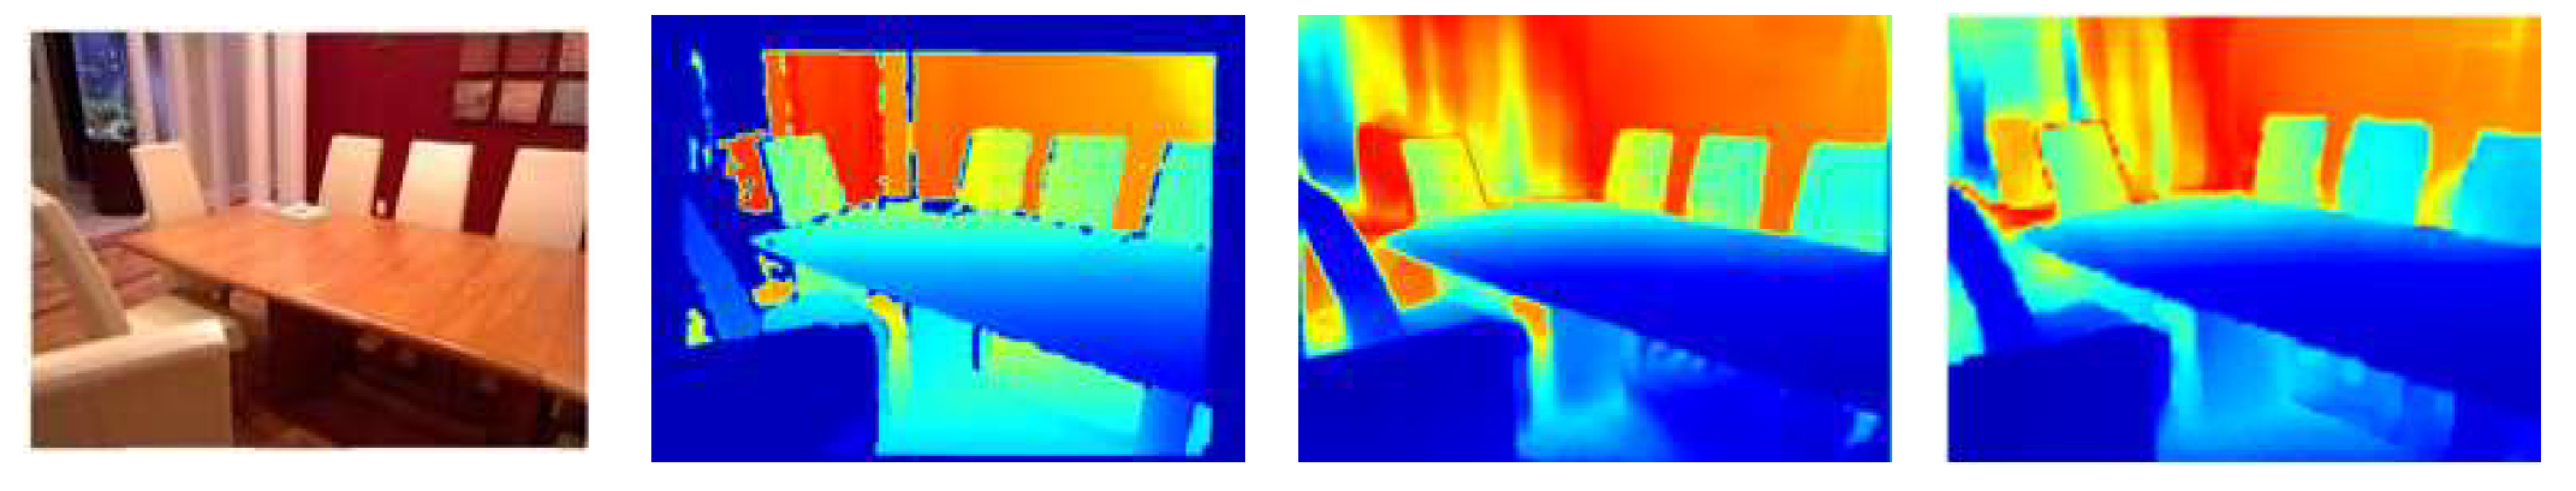
\includegraphics[width=.85\textwidth,angle=0]{figure 2-1.pdf}
    \caption{Stratégie riadenia navigácie v formácií.}
    \label{o:3}
\end{figure}

\subsubsection{Deliberatívne riadenie}
Prístup založený na plánovaní pohybu a trajektórie pohybu vyžaduje predbežné znalosti prostredia na plánovanie pohybov
robotov \citep{vascak}. Tento prístup využíva formalizmy ako Voronoiove diagramy alebo umelé potenciálne funkcie \citep{rimon},
pričom zohľadňuje všeobecné poznatky o životnom prostredí. Plánovanie pohybu je všeobecne optimálne z hľadiska
efektívnosti / reaktivity. V skutočnosti sa pre mierku veľmi veľkého počtu robotov nemodifikujú dobre kvôli výpočtovej
zložitosti. Vďaka predchádzajúcim znalostiam prostredia však roboti svoju misiu zvyčajne úspešne dokončia dobrým
výkonom.

\subsubsection{Reaktívne riadenie}
Pri reaktívnej metóde, roboty konajú iba podľa informácií svojich miestnych senzorov bez akýchkoľvek
ďalších všeobecných znalostí. Techniky založené na správaní sú vynikajúcou ilustráciou reaktívnej kontroly.
Globálna úloha robota je v skutočnosti rozdelená na súbor čiastkových úloh (vzorce správania).
Podľa informácií o senzore je stratégia riadenia použitá na robota založená na jednom zvolenom vzorci správania 
alebo je zlúčením niekoľkých vážených modelov. Keď aplikácia vyžaduje, aby roboty fungovali v reálnom čase (napríklad v nebezpečných
prostrediach), je zrejmé, že reaktívne metódy sa stávajú oveľa zaujímavejšími ako plánovanie pohybu \citep{vascak}.

\paragraph{Hierarchická stratégia.}
Pri prvom prístupe sa jeden alebo viac robotov považuje za vedúcich a iné roboti sú ďalší. Vedúci typicky sleduje danú
trajektóriu, zatiaľ čo nasledovníci sledujú jej transformované súradnice. Tento prístup sa dá ľahko sledovať.
Je však zaznamenané, že problém s hlavným robotom spôsobí zastavenie celého systému. V prístupe distribuovaného správania, 
neexistuje medzi robotmi hierarchia. Každý má svoje vlastné vnímanie a kontrolu a porucha robota nevedie k zlyhaniu
skupiny \citep{vascak}.

\paragraph{Stratégia správania.}
Stratégia založená na správaní znamená, že každý robot má súbor správania (základné úlohy), ktoré musia byť vykonané.
Výsledné skupinové správanie vyplýva zo základnej lokálnej interakcie bez explicitného vzoru celkového kooperatívneho
správania. Tento prístup však bol kritizovaný za to, ako volí riadenie pre každého robota. Podľa informácií o vnímaní
riadiaci systém v skutočnosti prepína medzi správaním (napríklad konkurenčný prístup) alebo kombinuje niekoľko
ovládačov (napríklad motorický obvod). To prirodzene sťažuje štúdium udržateľnosti stratégie globálneho riadenia \citep{ogren}.

\paragraph{Stratégia virtuálnej štruktúry.}
Virtuálna štruktúra (tretí prístup) považuje vzdelávanie za jediné virtuálne telo. Tvar posledného menovaného je
požadovaný tvar formácie a jeho pohyb sa prevedie na požadovaný pohyb každého vozidla. Virtuálna štruktúra
bola implementovaná v niekoľkých dielach s využitím potenciálnych metód poľa: teda všetky prvky formácie
sledujú pridelené uzly, ktoré prechádzajú do požadovanej konfigurácie. Na rozdiel od plánovania
pohybu využívajú potenciálne funkcie použité pri prístupe k virtuálnej štruktúre iba okamžité a lokálne vnímanie
robotov. Nedostatočné využitie potenciálnych prvkov pre tento druhý prístup zodpovedá zvyšujúcej sa zložitosti riadenia
tvaru flotily v dynamickom prostredí. To v skutočnosti znamená, že robot je vystavený často sa meniacemu počtu /
amplitúde síl, čo vedie k ďalším lokálnym minimám, fluktuáciám atď. Preto je v tomto prípade veľmi ťažké preukázať
spoľahlivosť a stabilitu navigácie \citep{ogren}, \citep{vascak}.



\subsection{Multi-robotické systémy podľa typovosti}
Skupinu robotov definujeme ako homogénnu, ak sú možnosti jednotlivých robotov rovnaké a inak skupina je heterogénna. Heterogenita
vo všeobecnosti prináša zložitosť, pretože alokácia úloh sa stáva zložitejšou a agenti majú väčšiu potrebu modelovať
ďalších robotov v skupine. Existuje koncept pokrytia úlohy, ktorý meria schopnosť daného člena tímu dosiahnuť danú
úlohu. Tento parameter predstavuje index dopytu po spolupráci: keď je pokrytie úloh vysoké, úlohy je možné splniť bez
väčšej spolupráce, ale inak je spolupráca nevyhnutná. Pokrytie úlohy je maximálne v homogénnych skupinách a klesá, keď
sú skupiny čoraz viac heterogénne (t. j. v krajnom prípade môže danú úlohu vykonať iba jeden agent v skupine).
V literatúre v súčasnosti prevládajú diela, ktoré predpokladajú homogénne skupiny robotov. Niektoré pozoruhodné
architektúry však dokážu zvládnuť heterogenitu, napr. ACTRESS a ALLIANCE. V heterogénnych
skupinách môže byť alokácia úloh určená individuálnymi schopnosťami, ale v homogénnych systémoch môže byť potrebné, aby
sa agenti diferencovali do rôznych rolí, ktoré sú vždy známe v čase návrhu alebo dynamicky vznikajú za behu \citep{vascak}.

\subsection{Komunikačné štruktúry}
Komunikačná štruktúra skupiny určuje možné spôsoby interakcie. Charakterizujeme tri základné typy interakcií, ktoré môžu
byť podporované.

\subsubsection{Interakcia prostredím}
Najjednoduchší typ interakcie sa vyskytuje, keď je samotné prostredie komunikačné médium (v skutočnosti,
zdieľanej pamäti) a medzi agentmi nie je explicitná komunikácia alebo interakcia. Niektorí výskumníci tiež nazývali túto
modalitu s "spoluprácou bez komunikácie" \citep{arkin}.

\subsubsection{Interakcia prostredníctvom snímania}
Interakcia prostredníctvom snímania patrí do miestnych interakcií, ktoré sa vyskytujú medzi agentami v dôsledku toho, že agenti sa navzájom cítia, ale bez
explicitnej komunikácie. Tento typ interakcie si vyžaduje schopnosť agentov rozlišovať medzi inými činiteľmi v skupine a
ďalších objektoch v prostredí, ktoré sa v niektorých literárnych zdrojoch nazýva "súvisiace uznanie" \citep{mataric}.
Interakcia prostredníctvom sondovania je potrebná na simuláciu iných agentov. Vzhľadom na obmedzenia hardvéru je
interakcia cez snímanie často emulovaná pomocou rádiovej alebo infračervenej komunikácie.

\subsubsection{Interakcia prostredníctvom komunikácie}
Tretia forma interakcie spočíva v explicitnej komunikácii s inými agentmi buď prostredníctvom zmenených, alebo
vysielaných zámerných správ (príjemca správy môže byť známy alebo neznámy). Pretože architektúry,
ktoré umožňujú túto formu komunikácie, sú podobné komunikačným sieťam, vzniká veľa štandardných problémov z oblasti
sietí, vrátane návrhu sieťových topológií a komunikačných protokolov. Napríklad na komunikáciu medzi robotmi
môže sa použiť prístupový protokol k médiám (podobný protokolu Ethernet). Aj som stretol komunikáciu pomocou protokolu
„hello-call“, pomocou ktorého ustanovujú „reťazce“ s cieľom rozšíriť svoje
efektívne komunikačné rozsahy a bezdrôtovým protokolom CSMA/CD (Carrier Sense Multiple Access with Collision Detection)
pre distribuované robotické systémy \citep{wang}.

\subsection{Vybrané typy architektúr}
Všetky systémy implementujú určitú skupinovú architektúru. Teraz popíšeme niekoľko obzvlášť dobre definovaných
reprezentatívnych architektúr spolu s prácami vykonanými v každom z ich rámcov. Je zaujímavé poznamenať, že tieto
architektúry zahŕňajú celé spektrum od tradičnej AI po vysoko decentralizované prístupy.

\subsubsection{CEBOT}
CEBOT (CEllular roBOTics System) je decentralizovaná, hierarchická architektúra inšpirovaná bunkovou organizáciou
biologických entít. Systém sa konfiguruje dynamicky  v tých základných autonómnych „bunkách“ (robotoch), ktoré je
možné fyzicky spojiť s inými bunkami, a dynamicky konfigurujú svoju štruktúru na „optimálnu“ konfiguráciu v reakcii na
meniace sa prostredia. V hierarchii CEBOT existujú „hlavné bunky“, ktoré koordinujú čiastkové úlohy a komunikujú s
ostatnými hlavnými bunkami \citep{michael} \citep{beatriz}.

\subsubsection{ACTRESS}
V systéme ACTRESS (robot a syntetický systém na báze ACTor) tvoria „roboti“ vrátane 3 robotov a 3 pracovných staníc
(jeden ako rozhranie k ľudskému operátorovi, jeden ako obrazový procesor a druhý ako globálny manažér prostredia)
heterogénnu skupinu, ktorá sa snaží vykonávať úlohy, ako je tlačenie objektov, ktoré nemôže vykonať žiadny z
robotov sám. Komunikačné protokoly na rôznych úrovniach abstrakcie poskytujú prostriedky, na ktorých
sú postavené mechanizmy „skupinového obsadenia“ a rokovacie mechanizmy založené na viacstupňových protokoloch vyjednávania. Študujú sa rôzne problémy, ako napríklad efektívna komunikácia medzi robotmi a manažérmi
prostredia, predchádzanie kolíziám \citep{beatriz}.

\subsubsection{SWARM}
SWARM je distribuovaný systém s veľkým počtom autonómnych robotov. (Upozorňujeme, že práca na systémoch SWARM sa
začala ako práca na bunkových robotických systémoch, kde mnoho jednoduchých agentov obsadzovalo jedno- alebo
dvojrozmerné prostredie a boli schopní vykonávať úlohy, ako je generácia vzorov a samoorganizácia). Inteligencia SWARM
je „vlastnosťou systémov neinteligentných robotov vykazujúcich kolektívne inteligentné správanie“. Samoorganizácia
v SWARM-e je schopnosť distribuovať sa „optimálne“ pre danú úlohu, napríklad prostredníctvom formovania geometrických
vzorov alebo štruktúrnej organizácie. SWARM vykazuje distribuovanú architektúru, zvyčajne bez rozdielov medzi členmi.
Interakcia prebieha tak, že každá bunka reaguje na stav \citep{beatriz}.

\subsubsection{GOFER}
Architektúra GOFER bola použitá na štúdium distribuovaného riešenia problémov viacerými mobilnými robotmi vo
vnútornom prostredí s využitím tradičných techník AI. V systéme GOFER centrálny systém plánovania a plánovania úloh
(CTPS) komunikuje so všetkými robotmi a má globálny prehľad o úlohách, ktoré sa majú vykonať, aj o dostupnosti robotov
na vykonávanie úloh. CTPS generuje štruktúru plánu (šablóna pre inštanciu plánu) a informuje všetkých dostupných robotov
o očakávaných cieľoch a štruktúrach plánu. Roboty používajú na určenie svojich rolí algoritmus prideľovania úloh \citep{caloud}.

\subsubsection{ALLIANCE}
Architektúru ALLIANCE vyvinul Parker \citep{parek} s cieľom študovať spoluprácu v heterogénnom, malom až strednom tíme
prevažne nezávislých a voľne prepojených robotov. Roboty sa považujú za schopné s určitou pravdepodobnosťou vycítiť
účinky ich vlastných činov a činov iných agentov prostredníctvom vnímania a explicitnej rozhlasovej komunikácie.
Jednotliví roboti sú založené na ovládači založenom na správaní s rozšírením pre aktiváciu „skupín správania“, ktoré
plnia určité úlohy. Tieto súbory sú aktivované motivačným správaním, ktorého aktivity sú určené robotovou
informovanosťou ich spoluhráčov \citep{beatriz} \citep{vascak}.


%
\section{Navrh}
V tejto časti sa budeme zaoberať návrhom nášho systému riadenia dronov vrátane hardvérových a softvérových komponentov a ich vzájomnej interakcie. Cieľom je poskytnúť komplexný prehľad návrhu systému vrátane technických špecifikácií a funkcií, aby ostatní mohli systém pochopiť a replikovať. Budeme tiež diskutovať o rôznych konštrukčných úvahách, ktoré boli súčasťou vývoja systému, a o tom, ako sme ich riešili.

\subsection{Výber dronu}
Po preskúmaní funkcií možných programovateľných dronov je najlepším zariadením kvadrokoptér Tello, ktorú vyvinula spoločnosť Ryze, ale podporuje ju spoločnosť DJI. Dron Tello je malý quadcopter určený na lietanie v interiéri, ktorý má procesor Intel. Má rozmery len 98 x 92,5 x 41 mm a váži len 87 gramov, čo uľahčuje jeho prepravu a manévrovanie v stiesnených priestoroch. Dron je vybavený 5 MP kamerou, ktorá dokáže zachytiť video s rozlíšením 720p pri 30 snímkach za sekundu, takže je vhodný na základné fotografovanie a videografiu. Má tiež optický snímač toku smerujúci nadol a infračervený snímač vzdialenosti, ktoré mu pomáhajú udržiavať stabilný let v interiéri.

\begin{figure}[ht!]
    \centering
    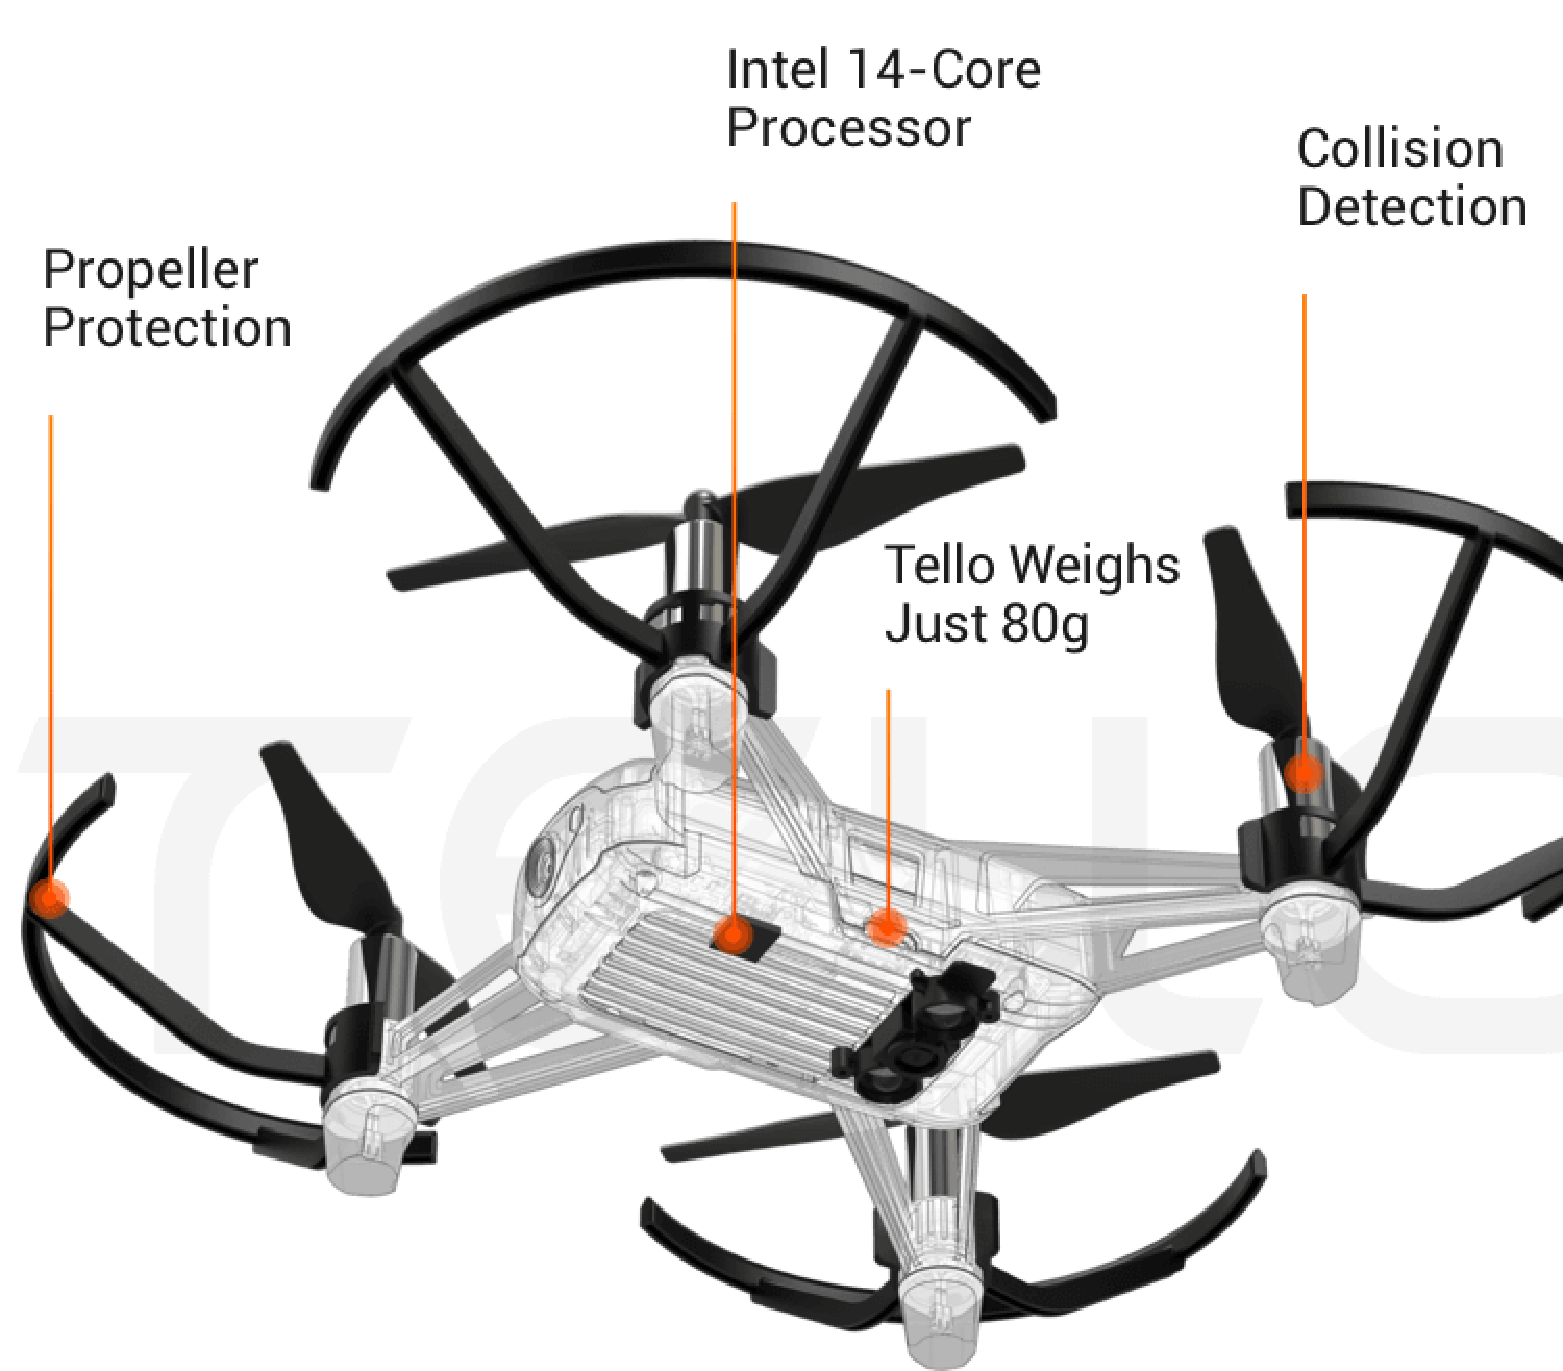
\includegraphics[width=.40\textwidth,angle=0]{figure 3-1.pdf}
    \caption{Dron DJI Tello a jeho komponenty.}
    \captionsetup{font=footnotesize, justification=centering, skip=5pt}
    \caption*{(Zdroj: www.ryzerobotics.com)}
    \label{o:3-1}
\end{figure} 

Dron Tello možno naprogramovať pomocou rôznych softvérových vývojových súprav (SDK). Jedným z populárnych SDK na programovanie dronu Tello je DJI Tello SDK, ktorý poskytuje súbor API na ovládanie letu, kamery a ďalších funkcií dronu. Súbor Tello SDK je k dispozícii pre viaceré programovacie jazyky vrátane jazykov Python, Java a Swift, vďaka čomu je prístupný vývojárom s rôznym vzdelaním a úrovňou zručností \citep{TelloSDK}.

Okrem DJI Tello SDK je k dispozícii aj niekoľko SDK a knižníc tretích strán na programovanie dronu Tello vrátane knižnice TelloPy pre Python a knižnice Node.js Tello pre Node.js. Tieto knižnice poskytujú ďalšie funkcie na ovládanie dronu a spracovanie údajov z jeho senzorov a môžu byť užitočné pre pokročilejšie projekty .

Celkovo je dron Tello všestrannou a cenovo dostupnou možnosťou pre interiérové aplikácie dronov a jeho podpora viacerých programovacích jazykov a SDK ho sprístupňuje vývojárom s rôznym vzdelaním a úrovňou zručností. 

\subsection{Programovací jazyk a súbor nástrojov}
Systém je založený na webovej aplikácii vyvinutej pomocou React, ktorá umožňuje používateľom ovládať drony v reálnom čase. Webová aplikácia komunikuje s backendovým serverom vytvoreným pomocou Node.js, ktorý funguje ako sprostredkovateľ medzi používateľom a dronmi \citep{TelloSDK}.

Frontend webovej aplikácie je vytvorený pomocou React, populárnej JavaScriptovej knižnice na vytváranie používateľských rozhraní. React umožňuje vytvárať opakovane použiteľné komponenty používateľského rozhrania, ktoré možno ľahko spravovať a aktualizovať. Okrem React využíva frontend aj ďalšie webové technológie, ako sú HTML5 a CSS3 \citep{TelloSDK}.

Backendový server je vytvorený pomocou Node.js, populárneho prostredia na spúšťanie JavaScriptu. Node.js umožňuje vytvárať škálovateľné a vysoko výkonné sieťové aplikácie, preto je vhodnou voľbou na vybudovanie backendu systému. Backendový server komunikuje s frontendom prostredníctvom rozhraní RESTful API a spojení WebSocket.

\begin{figure}[ht!]
    \centering
    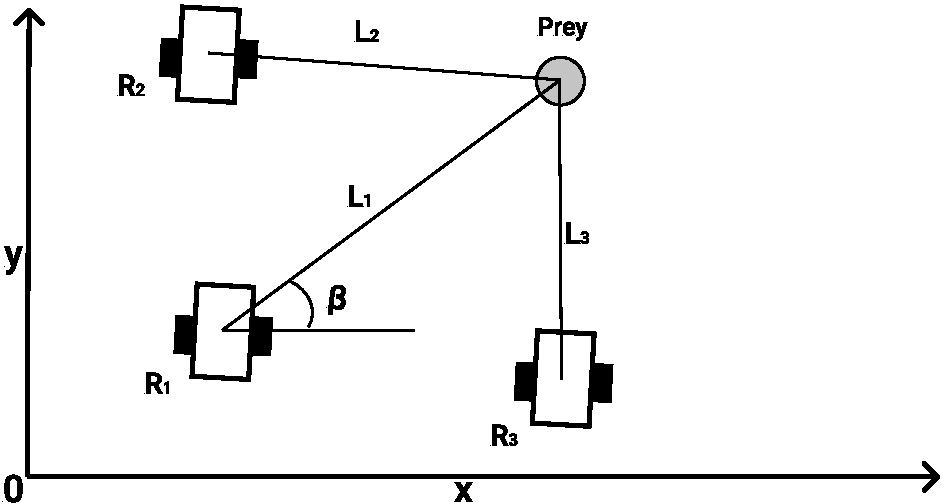
\includegraphics[width=.90\textwidth,angle=0]{figure 3-2.pdf}
    \caption{Schéma návrhu systému: Webová aplikácia vytvorená pomocou React komunikuje s backendovým serverom Node.js, ktorý posiela príkazy a prijíma telemetrické údaje z dronov pripojených k ASUS Tinkerboard.}
    \captionsetup{font=footnotesize, justification=centering, skip=5pt}
    \caption*{(Zdroj: vlastné spracovanie)}
    \label{o:3-2}
\end{figure}  

Na ovládanie dronov a prijímanie ich telemetrických údajov je backendový server pripojený k doske ASUS Tinker Board. Tinker Board je výkonný jednodoskový počítač, na ktorom beží upravená verzia systému Linux. Na každej doske Tinker Board je pre každý dron spustený program v jazyku Python. Tieto programy v jazyku Python sú zodpovedné za prijímanie príkazov z backendového servera a ich odosielanie do dronov, ako aj za prijímanie telemetrických údajov z dronov a ich odosielanie späť na backendový server.

Nakoniec systém využíva aj značky Aruco na zisťovanie polohy a orientácie dronov, ktoré sa používajú na riadenie pohybu dronov. Detekcia a sledovanie značiek Aruco sa vykonáva pomocou populárnej knižnice počítačového videnia OpenCV. Systém je tiež vybavený kamerou namontovanou na každom drone, ktorá zachytáva živý videozáznam, ktorý sa v reálnom čase prenáša späť do webovej aplikácie pomocou WebSocketov.
\subsection{Ako ovládať dron tello}
V dokumentácii poskytnutej výrobcom je podrobne opísané, ako ovládať dron pomocou programu Python. [19] Po pripojení k vlastnej sieti wifi dronu je potrebné otvoriť spojenie UDP na ovládanie dronu prostredníctvom adresy 192.168.10.1 a portu 8889. Pred spustením ovládania je vždy potrebné poslať dronu príkaz "command", ktorý sa prepne do stavu, v ktorom čaká na príkazy \citep{TelloSDK}. 
Z dronu je tiež možné čítať stav letového ovládača, ktorý využíva aj firmvér zariadenia, otvorením servera 0.0.0.0 na porte 8890. Ten nebol súčasťou vyššie uvedenej knižnice GitHub, preto sme ho do programu pridali. Otvorili sme nové spojenie so soketom UDP so spomínaným serverom a údajmi na porte bežiacim v samostatnom vlákne, podobne ako pri prijímaní odpovedí z kontroly dronu na pozadí. 

\begin{mypython}[caption={ukazuje obsluhu vlákna obsiahnutú v jazyku Python },label=SO-test]
    # Run Tello command responses UDP receiver on background
    client_socket = socket.socket(socket.AF_INET,socket.SOCK_DGRAM)
    response_receiver_thread = Thread(target=Tello.udp_response_receiver)
    response_receiver_thread.daemon = True
    response_receiver_thread.start()

    # Run state UDP receiver on background
    state_receiver_thread = Thread(target=Tello.udp_state_receiver)
    state_receiver_thread.daemon = True
    state_receiver_thread.start()

    threads_initialized = True
\end{mypython} 

  

Threading library, ktorý možno priradiť konkrétnej funkcii, 
ktorá bude bežať na vlákne oddelenom od hlavného programu. 
Vlákno, ktoré číta stav, ukazuje na funkciu get$_-$read$_-$state()
triedy Tello a spúšťa ju v samostatnom vlákne, takže beží na pozadí. Mali by ste zapnúť voľbu daemon = True, aby sa 
vlákno spúšťalo ako daemon, t. j. ak sa ukončí program vyššej úrovne, ukončí sa aj vlákno daemon. Ak táto možnosť nie 
je zapnutá, budete musieť ukončenia vlákien riešiť samostatne \citep{TelloSDK}.

Stavy vysiela dron na spomínanom serveri, ich čítanie nebude spomaľovať čítanie obrazu z kamery dronu, pretože dron bude vysielať reťazec stavov po vstupe do príkazového režimu, aj keď ho nebudeme čítať. V oficiálnej dokumentácii je uvedený formát, v ktorom dron vysiela stavy svojich senzorov. Vysiela jeden súvislý, stredníkmi ohraničený textový súbor ASCII cez bezdrôtové spojenie UDP na prijímajúci server v nasledujúcom formáte: \pyth{"pitch:%d;roll:%d;yaw:%d;vgx:%d;vgy:%d;vgz:%d;templ:%d;temph:%d;tof:%d;h:%d;bat:%d; baro:%.2f;time:%d;agx:%.2f;agy:%.2f;agz:%.2f;\r\n"}
Kde sú uvedené hodnoty jednotlivých stavov (interpretácia súradníc je uvedená na obrázku 8):
\begin{itemize}
\item \textbf{pitch, roll, yaw}: vlastná rotácia dronu okolo osí x, y a z, meraná ako celý uhol, kladný v smere hodinových ručičiek, podľa pravidla ľavej ruky;
\item \textbf{vgx, vgy, vgz}: rýchlosť dronu nastavená v smeroch x, y, z v cm/s (nie sú to skutočné merateľné hodnoty rýchlosti, ale hodnota priradená k rýchlosti dronu, ktorá sa mení počas riadenia);
\item \textbf{temp}: najnižšia teplota v C°; 
\item \textbf{temph}: najvyššia teplota v C° 
\item \textbf{tof}: výška kamery času letu v cm v spodnej časti dronu; 
\item \textbf{h}: výška v cm; 
\item \textbf{bat}: zostávajúca kapacita batérie dronu v celých percentách; 
\item \textbf{baro}: hodnota výšky na základe nainštalovaného barometra v cm; 
\item \textbf{time}: čas zapnutia motorov (čas letu) v sekundách; 
\item \textbf{agx, brain, agz}: zrýchlenie dronu v smere x, y, z zo snímača zrýchlenia interpretované v 0,001 g, kde g je gravitačné zrýchlenie. 
\end{itemize}

Toto sa dá rozdeliť na pole pozdĺž stredníkov pomocou funkcie Python string.split("; ") a potom sa hodnoty za dvojbodkou v poli prevedú na číselný typ v príslušnom formáte. Na číslo sa prevedú len požadované hodnoty a potom sa hodnoty načítajú do zoznamu, ktorý sa odovzdá do riadku. V Pythone je v rámci obsluhy vlákien len typ Queue, schopný zabezpečiť bezpečnu komunikáciu medzi vláknami; ak sa nepoužíva na výmenu údajov medzi vláknami v programe, program môže zamrznúť. 
\begin{mypython}[caption={Funkcia na čítanie stavov dronov },label=CL-2]
def get_read_state(self): 
    while True: 
        time.sleep(1/25) 
        try: 
            state_temp, _ = self.stateSocket.recvfrom(1024) 
            self.state = state_temp.decode('ASCII'). split(";") 
            pitch = -int(self.state[0][self.state[0].index(":")+1:]) 
            roll = -int(self.state[1][self.state[1].index(":")+1:]) 
            yaw = -int(self.state[2][self.state[2].index(":")+1:]) 
            tof = int(self.state[10][self.state[8].index(":")+1:]) 
            bat = int(self.state[10][self.state[10].index(":")+1:]) 
            self.data_queue.put([pitch, roll, yaw, tof, bat]) 
        except Exception as e: 
            self.LOGGER.error(e) 
\end{mypython} 
Počas riadenia máte tiež možnosť čítať stav tak, že pošlete do vlákna dotaz ako príkaz, na ktorý odpovie prostredníctvom spojenia UDP. Tieto dotazové slová poskytujú rovnaké stavy senzorov ako čítanie stavu (napr. : "akcelerácia?", "rýchlosť?", "batéria?", "tof?" ...). Zvažovalo sa aj použitie tejto funkcie, ale testy ukázali, že táto metóda poskytuje menej spoľahlivé výsledky. Táto komunikácia, na rozdiel od čítania stavu, spomaľuje a preťažuje ostatné funkcie dronu, pretože na reakciu na ne musí zabezpečiť samostatnú procesorovú kôru. Keďže teda nemôžeme získať spoľahlivé rezultáty ani s obsluhou vlákien, táto funkcia nie je pre naše účely užitočná. 

Obraz z kamery, ktorý je pre túto úlohu nevyhnutný, sa tiež vysiela cez UDP, pričom sa otvorí server 0.0.0.0 cez port 11111 \citep{Virbora2022}. Keďže veľkosť zakódovaných údajov obrazu je väčšia ako maximálna veľkosť užitočného zaťaženia prenosu UDP, obrazové údaje dron prenáša v blokoch po 1460 bajtov, z ktorých posledný blok je menší ako 1460 bajtov. Vysielaný obraz je možné po prijatí zobraziť pomocou balíka OpenCV. Balíky kodekov ffmpeg a libh264decoder uvedené v oficiálnej dokumentácii DJI-SDK preto v tomto prípade nie sú potrebné, testovanie programu prebieha pod operačným systémom MacOS \citep{Virbora2022}. 
Ovládacie inštrukcie SDK možno rozdeliť do troch skupín: 
\begin{enumerate}
\item inštrukcie na riadenie 
\begin{enumerate}
    \item vrátenie 'ok', ak sú splnené 
    \item "error" alebo chybové hlásenie, ak nie je 
\end{enumerate}
\item inštrukcie na čítanie 
\begin{enumerate}
    \item vráti hodnotu požadovaného parametra
\end{enumerate}
\item ovládanie nastavením parametrov 
\begin{enumerate}
    \item vrátenie 'ok', ak sú splnené 
    \item 'error' alebo chybové hlásenie, ak nie je 
\end{enumerate}
\end{enumerate}



Dronovi sa pošle príkaz "\pyth{takeoff}" (vzlet), vzlietne, pristane na príkaz "\pyth{land}" (pristátie), príkazy "\pyth{streamon}" (zapnutie) a "\pyth{streamoff}" (vypnutie) na prepnutie streamovania videa. Samotný dron je možné ovládať podľa smeru a súčasne príkazom "\pyth{go x y z speed}" (Obrázok 3-3). V tomto prípade sa dron bude pohybovať zadanou rýchlosťou vzhľadom na danú polohu v smere určenom tromi súradnicami. Presnosť tohto ovládania sa rovná rozmerom dronu, takže sa nemôže pohybovať o menej ako 20 centimetrov \citep{TelloSDK}. 

\begin{figure}[ht!]
    \centering
    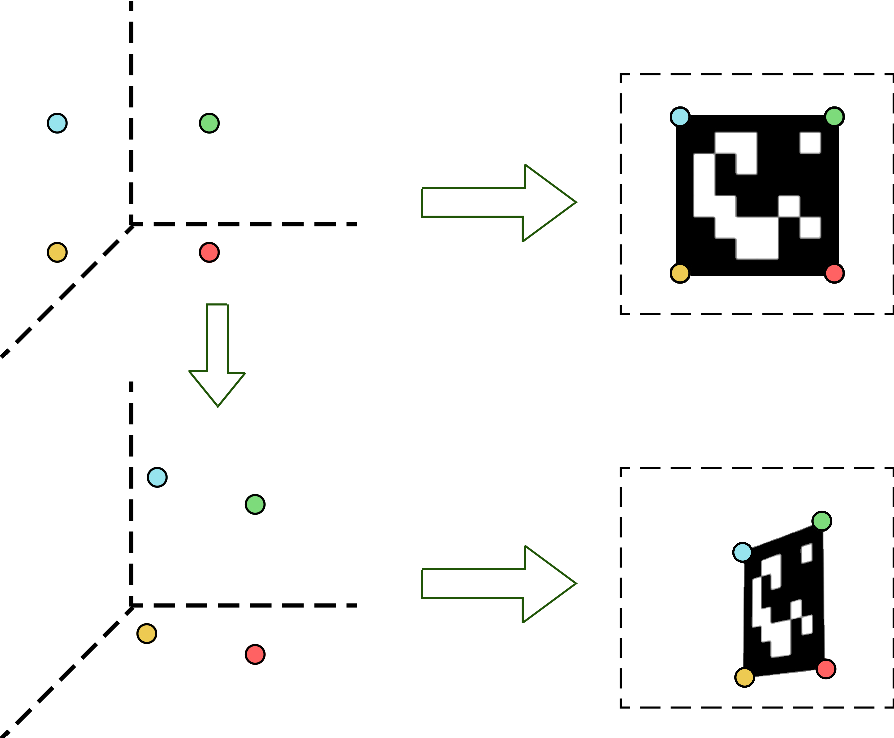
\includegraphics[width=.55\textwidth,angle=0]{figure 3-3.pdf}
    \caption{Smery definované pri ovládaní dronu pomocou SDK.}
    \captionsetup{font=footnotesize, justification=centering, skip=5pt}
    \caption*{(Zdroj: vlastné spracovanie)}
    \label{o:3-3}
\end{figure}  
Firmvér poskytuje aj možnosť ovládať dron v oblúku: zadaním ďalších dvoch bodov so súradnicami x, y, z vzhľadom na aktuálnu polohu dronu opíše nimi definovaný oblúk, ak je polomer oblúka v rozmedzí 0,5 až 10 metrov.

Pre túto úlohu je na základe testov s dronom najvhodnejším spôsobom riadenia tzv. RC riadenie, ktoré patrí do skupiny 3 spôsobov riadenia. Rýchlosti dronu v smeroch x, y, z a odklonu možno nastaviť príkazom "\pyth{rc x y z yaw}". S celočíselnými hodnotami od -100 do 100. (Rýchlosť yaw je tu tiež vyjadrená v súradnicovom systéme bal offset). Takto môžete dokonca vykresliť krivku odoslaním príkazov s danou frekvenciou za predpokladu, že hodnoty rýchlosti parametrickej krivky sú en- tované ako kontrola vzorkovaním s rovnakou frekvenciou. Pri tomto režime riadenia možno dosiahnuť menšie posuny ako pri už spomínaných príkazoch "go x y z speed". 
Do 2. skupiny inštrukcií patria inštrukcie, ktoré sa pýtajú na údaje zo senzorov. Napríklad aktuálne nastavenú rýchlosť, nabitie batérie, čas letu, nadmorskú výšku, zrýchlenie a uhlovú rýchlosť možno načítať z palubného ovládača dronu. Tieto sa nepoužívajú z dôvodu nespoľahlivej čitateľnosti, ktorá bola spomenutá vyššie \citep{TelloSDK}.

\subsection{Umiestnenie dronu}
Na zabezpečenie presného a spoľahlivého ovládania dronov je nevyhnutné optimálne umiestnenie dronov a značkovačov Aruco. Drony by mali byť umiestnené na otvorenom priestranstve s minimom prekážok a jasnou viditeľnosťou na značky. Značky by mali byť umiestnené tak, aby umožňovali maximálne pokrytie záujmovej oblasti a zároveň boli ľahko zistiteľné kamerou dronu.

Je tiež dôležité zabezpečiť, aby boli značky umiestnené v rovnakej výške a orientácii, čo uľahčí presnú detekciu a sledovanie. Do úvahy by sa mali brať aj akékoľvek zmeny svetelných podmienok, pretože môžu ovplyvniť detekciu a sledovanie značiek.

Okrem fyzického umiestnenia je tiež dôležité správne kalibrovať nastavenia dronu a kamery. To zahŕňa nastavenie parametrov, ako je rozlíšenie kamery, ohnisková vzdialenosť a korekcia skreslenia, aby sa zabezpečilo presné meranie a umiestnenie.

Dôkladným zvážením všetkých týchto faktorov možno umiestnenie dronu optimalizovať tak, aby sa dosiahol čo najlepší výkon a presnosť pre danú aplikáciu.

Údaje o zrýchlení by sa mohli použiť na určenie polohy, ale po odoslaní príkazu "zrýchlenie?" dáva čítanie veľmi nejasnú odpoveď. Dokonca aj po zmene časového limitu spojenia na požiadavku odosielanú s intervalom 0,1 sekundy nastaveného počas testov, stále dával zmysluplnú odpoveď po 0,5 sekundy, ale často len vyhadzoval chybu timeout. Takto boli prirodzene zašumené údaje akcelerometra načítané dokonca so značným vzorkovacím šumom. 

Druhou možnosťou je otvoriť server bežiaci v samostatnom vlákne, ktorý bude prijímať už spomínané stavové údaje. V tomto prípade dostávate údaje v jednom reťazci vrátane údajov akcelerometra a gyroskopu. Tieto údaje by bolo potrebné najprv prehnať cez ďalší filter \citep{7859621} alebo Kalmanov filter \citep{8839496} na odstránenie šumu zo senzorov. Dvojnásobnou integráciou hodnôt zrýchlenia možno získať posun dronu, ale integračná operácia zosilňuje šum, podlieha integračnej chybe a nedá sa korigovať v prípade absencie stabilných bodov polohy. Táto možnosť bola zavrhnutá z dôvodu akumulácie šumu pri integrácii. 

Preto sa vybrali značky ArUco, na základe ktorých možno merať relatívny posun kamery. Problémom pri nich je, že údaje o polohe možno získať len vtedy, keď je značka jasne viditeľná v obraze kamery. Tento problém sa však dá vyriešiť správnym označením testovacej plochy. Na umiestnenie značiek by sa mali použiť vhodné pravidlá, ktoré boli sformulované v časti 2.2.4, a tak možno určiť polohu kamery. 

\subsubsection{Používanie značkovačov aruco}
Funkcie potrebné na generovanie značiek ArUco nájdete v balíku prídavných modulov OpenCV-Contrib. Ich umiestnenie si vyžaduje kalibráciu kamery, ktorú možno vykonať aj pomocou kalibračného algoritmu v OpenCV na základe štúdie Z. Zhanga \citep{888718} odhadom parametrov kamery. 

Na kalibráciu potrebujete šachovnicu s dĺžkami strán, číslami riadkov a stĺpcov jej políčok. Na základe týchto údajov algoritmus vygeneruje teoretickú mapu vnútorných rohových bodov štvorcov a potom na základe vzoriek kamery vypočíta vnútorné a vonkajšie vlastnosti kamery v transformačných maticiach. Matica fotoaparátu obsahuje päť vnútorných vlastností fotoaparátu vrátane ohniskovej vzdialenosti, pomeru strán obrazového snímača a hlavného bodu dierkovej komory mod- elu. Získava sa aj matica skreslenia objektívu spojená s nelineárnymi vnútornými vlastnosťami, ktorú možno použiť na odstránenie súdkovitého a poduškovitého skreslenia na okrajoch obrazu. Vonkajšie (vonkajšie) vlastnosti kamery sú tiež opísané transformačnou maticou, ktorá realizuje prevod zo súradníc reálneho 3D priestoru na 3D súradnice kamery(Obrázok 3-5). Matica aplikuje homogénnu transformáciu: posun do stredu (počiatku) snímača kamery o vektor T a rotáciu o maticu rotácie R. 

\begin{figure}[ht!]
    \centering
    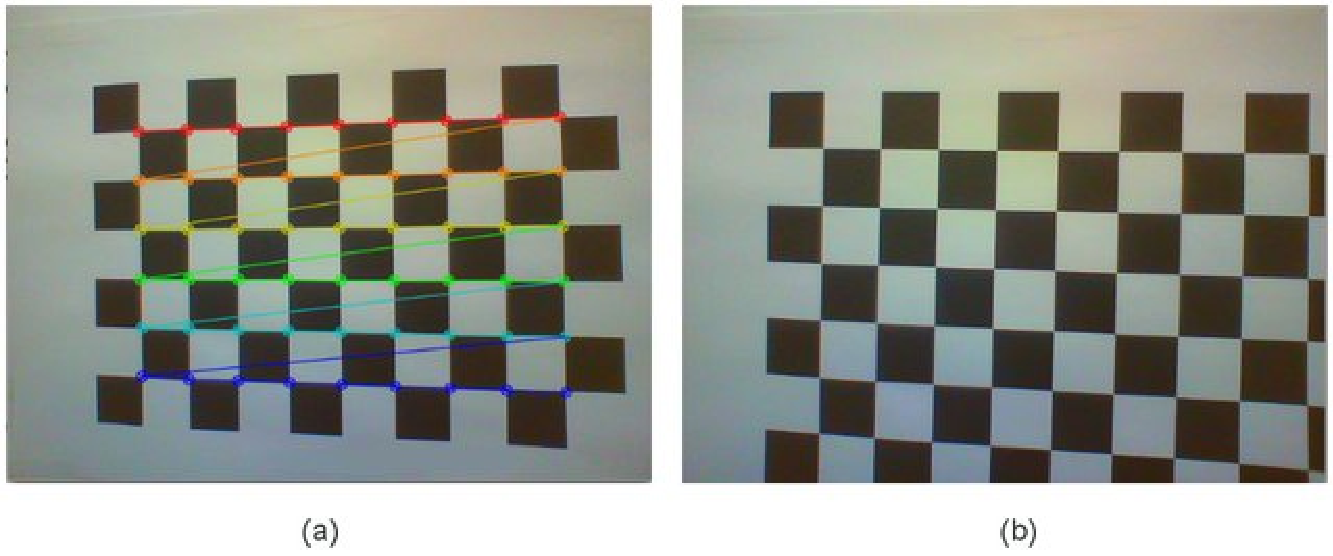
\includegraphics[width=.90\textwidth,angle=0]{figure 3-4.pdf}
    \caption{Tradičná kalibrácia pomocou vzoru šachovnice. a) Rutiny OpenCV dokážu odhaliť všetky rohy šachovnice. b) Rohy nemožno priradiť k príslušným bodom na vzore šachovnice, ak vzor nie je úplne zachytený.}
    \captionsetup{font=footnotesize, justification=centering, skip=5pt}
    \caption*{(Zdroj: vlastné spracovanie)}
    \label{o:3-4}
\end{figure}  

\begin{figure}[ht!]
    \centering
    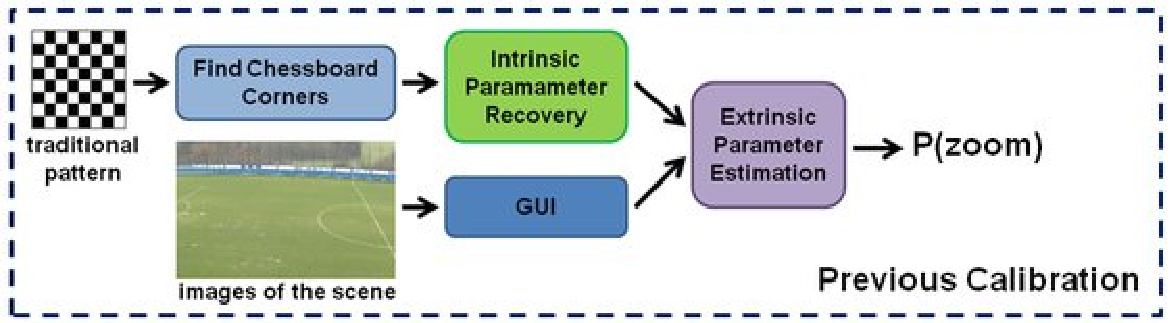
\includegraphics[width=.90\textwidth,angle=0]{figure 3-5.pdf}
    \caption{Schéma procesu kalibrácie.}
    \captionsetup{font=footnotesize, justification=centering, skip=5pt}
    \caption*{(Zdroj: vlastné spracovanie)}
    \label{o:3-5}
\end{figure}  

Teoreticky by na správnu kalibráciu mali stačiť dve vzorky, ale na dosiahnutie presnejších údajov pracujeme s 20 súbormi údajov. Fotografia na obrázku 3-4 bola zhotovená počas procesu kalibrácie. Výsledné matice sa ukladajú do súboru s názvom camcalib.npz a čítajú sa z neho, aby sa pred každým použitím nemusela kalibrovať zabudovaná kamera dronu. 

Jedným z najčastejších zdrojov chýb pri meraní kamerou je súdkovité skreslenie, ktoré možno odstrániť pomocou matice skreslenia získanej počas kalibrácie pomocou vstavanej funkcie OpenCV cv2.undistort(). Tým sa zníži efekt rybieho oka a do určitej miery sa zmenší zorné pole, ale získajú sa presnejšie hodnoty na okrajoch obrazu pre následné umiestnenie pomocou značiek ArUco.
\subsubsection{Pravidlá umiestňovania značiek}
Pri používaní značkovačov Aruco na určovanie polohy dronov je potrebné dodržiavať niekoľko dôležitých pravidiel, aby sa zabezpečili presné a spoľahlivé výsledky. Tu je niekoľko pokynov pre umiestnenie značiek \citep{Marut2019}:
\begin{enumerate}

\item \textbf{Dostatočný počet značiek}: Na presné sledovanie polohy a orientácie dronu je dôležité použiť dostatočný počet značiek. To pomôže zabezpečiť, aby boli značky vždy viditeľné z pohľadu dronu, aj keď sa dron rýchlo pohybuje;

\item \textbf{Značky umiestnite do mriežky}: Umiestnenie značiek do pravidelnej mriežky pomôže zabezpečiť ich rovnomerné rozloženie a viditeľnosť z viacerých uhlov. To môže tiež pomôcť znížiť pravdepodobnosť zákrytov alebo iných problémov, ktoré by mohli narušiť sledovanie;

\item \textbf{Vyber veľkosti značiek}: Veľkosť použitých značiek bude závisieť od vzdialenosti, z ktorej sa na ne bude pozerať. Napríklad, ak bude dron lietať relatívne blízko značiek, môžete použiť menšie značky. Ak však bude dron vo väčšej vzdialenosti, možno budete musieť použiť väčšie značky, aby ste zabezpečili viditeľnosť;

\item \textbf{Reflexný alebo priehľadný povrch}: Reflexné alebo priehľadné povrchy môžu narušiť detekciu značiek tým, že spôsobujú odrazy alebo lomy, ktoré skresľujú vzhľad značky. Aby ste sa vyhli tomuto problému, vyberte si miesto na umiestnenie značky, ktoré je bez reflexných alebo priehľadných povrchov;

\item V zornom poli dronu musí byť vždy prítomný aspoň jedna značka, aby sa zabezpečilo, že dron môže nepretržite sledovať svoju polohu a orientáciu;

\item Keď sa značky časom zistia a stratia, systém použije polohu a orientáciu predchádzajúceho značky na odhad aktuálnej polohy a trajektórie dronu, kým sa nezistí novu značku.
\end{enumerate}


\subsection{Prvé testy polohovania pomocou značiek}
Na testovanie sa použili štyri značky 7x7 ArUco s dĺžkou strany 0,0957 m z knižnice DICT-7x7-100. K dispozícii sú aj značky s plochami 4x4, 5x5 a 6x6, ale vyššie rozlíšenie knižnice 7x7 umožňuje presnejšie určovanie polohy. V každej knižnici je k dispozícii až 1024 rôznych značiek, čo by malo stačiť na poskytnutie informácií potrebných na riadenie dronu.

Odporúča sa používať viac ako jedna značka, pretože systém dokáže spriemerovať z viacerých hodnôt, takže spriemerovaním možno získať presnejšie výsledky, jednoducho odfiltrovaním akýchkoľvek odľahlých hodnôt. Okrem toho, ak je v zornom poli dronu niekoľko značiek, je menší problém, ak sa jedna z nich stratí, pretože stále môže čítať hodnoty z ostatných. V prvom experimente boli značky umiestnené kolmo na kameru dronu, vertikálne k stene, ako je znázornené na fotografii na obrázku 10. Cieľom tohto testu bolo zistiť, ako dobre dokáže softvér ukladať údaje, ktoré sa približujú realite.

Súbor bodov vľavo na obrázku 11 ukazuje, že súbor meracích bodov bol úspešne sledovaný hneď po opísaní štvorca dronom a dokonca aj po zakreslení jednej z jeho uhlopriečok, a vpravo ukazuje, že aj zmena výšky bola pomocou značiek zistená s vynikajúcou presnosťou. Priesečník čiernych osí je počiatok pohybu dronu. Body na obrázku vyznačené červenou farbou sú skutočné hodnoty a zelená krivka je B-spline krivka prispôsobená bodu nastavenému funkciou splprep() v podadresári interpolate balíka Scipy dostupného v programovacom jazyku Python. Parameter spresnenia funkcie bol po niekoľkých experimentoch na základe dokumentácie \citep{scipy-docs} zvolený na hodnotu s=0,1, čo al- ready dostatočne aproximuje množinu bodov odfiltrovaním zašumených bodov. Nakoniec sme vo finálnej verzii programu použili na filtrovanie dátových bodov Kalmanov filter namiesto metódy B-spline interpolácie, pričom sme mysleli na budúcu implementáciu v reálnom čase a adaptívnejšie správanie Kalmanovho filtra. 

Jediná korekcia, ktorú bolo potrebné aplikovať na experimentálnu sadu bodov, bolo negatívne otočenie bodov o 10,5° okolo osi x, inak by sa Z-koordináty bodov zväčšili, keď by sa približovali k značkám, a to aj pri konštantnej výške. Je to spôsobené uhlom kamery od vodnej hladiny, pričom pri priblížení k markerom sa zistila vyššia poloha. (Toto bude neskôr zbytočné kvôli korekcii uhlového natočenia značiek.)

V tomto nastavení bude dron poskytovať skutočné hodnoty posunutia len vtedy, ak je rovina kamery (okrem uhla poklesu) rovnobežná s rovinou značiek. Ak sa poloha od tejto odchýli, dron bude udávať nesprávne hodnoty. Hodnoty posunutia sa musia odhadnúť s prihliadnutím na uhly natočenia, inak nemôžeme previesť hodnoty vektorov translácie značiek ArUco do súradnicového systému prvej videnej značky, ktorý chceme použiť ako globálny súradnicový systém.  Hodnoty vektorov zadané funkciou cv2.aruco.estimatePoseSingleMarkers() balíka OpenCV sú zadané v súradnicovom systéme kamery, ktoré je potom potrebné previesť do súradnicového systému značiek. 

\subsubsection{Vyhodnotenie testu a očakávania od systému}
Na základe prvých testov sa oplatí ďalej skúmať túto možnosť určovania polohy, pretože dokáže vypočítať polohu dronu v reálnom čase s relatívne malým počtom transformácií. Bohužiaľ, nemôžeme využiť grafickú akceleráciu balíka CUDA, ktorú poskytuje spoločnosť Nvidia, pretože funkcie balíka OpenCV-Python neboli všetky pridané do knižnice cv2.cuda v jazyku Python. Spomalí to spracovanie obrazu, ale aj tak spôsobí väčšie oneskorenie operácie kvôli 1,5...2 sekundovému oneskoreniu kamerového obrazu prenášaného dronom. 

Očakáva sa, že chyba merania metódy bude približne 0,05 m pri zväčšenej veľkosti značiek a vhodnom počte značiek. V dôsledku konverzií medzi súradnicovými systémami značiek však môžeme očakávať aj chybu driftu, ktorá sa zvyšuje so vzdialenosťou od značky reprezentujúceho globálnu súradnicu v dôsledku nepresnosti transformácií medzi súradnicovými systémami.

\subsection{Princíp, spresnenie a robustnosť polohovania}
Počas vývojovej a testovacej fázy kamerového programu sme namiesto palubnej kamery dronu Tello použili webovú kameru. Dôvodom bola predovšetkým obmedzená životnosť batérie dronu, ktorá by sťažila testovanie a zdokonaľovanie programu na dlhší čas. Namiesto toho sme použili webovú kameru namontovanú na stabilnej platforme, ktorá simulovala pohľad kamery dronu, a testovali sme výkon programu v rôznych svetelných podmienkach, vzdialenostiach a orientáciách. Keď sme boli s výkonom programu spokojní, preniesli sme ho do dronu Tello a podľa potreby sme vykonali drobné úpravy.
Program bol napísaný s použitím funkcií poskytovaných v balíku OpenCV ArUco, napríklad:
\begin{enumerate}
\item \textbf{Detekcia a rozpoznávanie značiek}: Na detekciu a rozpoznanie značiek Aruco vo videokanáli dronu používame funkciu cv2.detectMarkers(). Táto funkcia prijíma obraz, slovník Aruco a parametre na detekciu a vracia zistené značky a ich príslušné ID;
\item \textbf{Transformácie medzi súradnicovými systémami značky a kamery}: Po zistení a rozpoznaní značiek musíme transformovať ich polohu v obraze (v pixelových súradniciach) na ich polohu v súradnicovom systéme kamery (v milimetroch). Toto sa vykoná pomocou funkcie cv2.aruco.estimatePoseSingleMarkers(), ktorá prijme detekované značky, veľkosť značiek, maticu kamery a koeficienty skreslenia a vráti vektory rotácie a translácie, ktoré predstavujú polohu každej značky v súradnicovom systéme kamery;
\item \textbf{Spresnenie pozícií značiek}: Keďže zistené polohy značiek nie sú vždy presné, musíme ich spresniť pomocou subpixelovej presnosti. To sa vykonáva pomocou funkcie cv2.cornerSubPix(), ktorá prijíma obraz, zistené rohy značky a parametre pre subpixelové spresnenie a vracia spresnené rohové pozície;
\item \textbf{Robustnosť polohovania}: Aby sme zabezpečili robustnosť a presnosť polohy dronu, používame v obraze viacero značiek a vykonávame priemerovanie ich polôh. To pomáha znížiť vplyv šumu a chýb pri detekcii a rozpoznávaní značiek;
\item \textbf{Transformácia perspektívy a bodu (PnP)}: Funkcia cv2.aruco.solvePnP() sa používa na odhad pózy (polohy a orientácie) značky v 3D priestore. Táto funkcia prijíma ako vstup 2D súradnice značky na obrázku, 3D súradnice značky v reálnom svete a maticu kamery, ktorá obsahuje vlastné parametre kamery (ohniskovú vzdialenosť, hlavný bod atď.) \citep{9549863}.
\end{enumerate}

\begin{figure}[ht!]
    \centering
    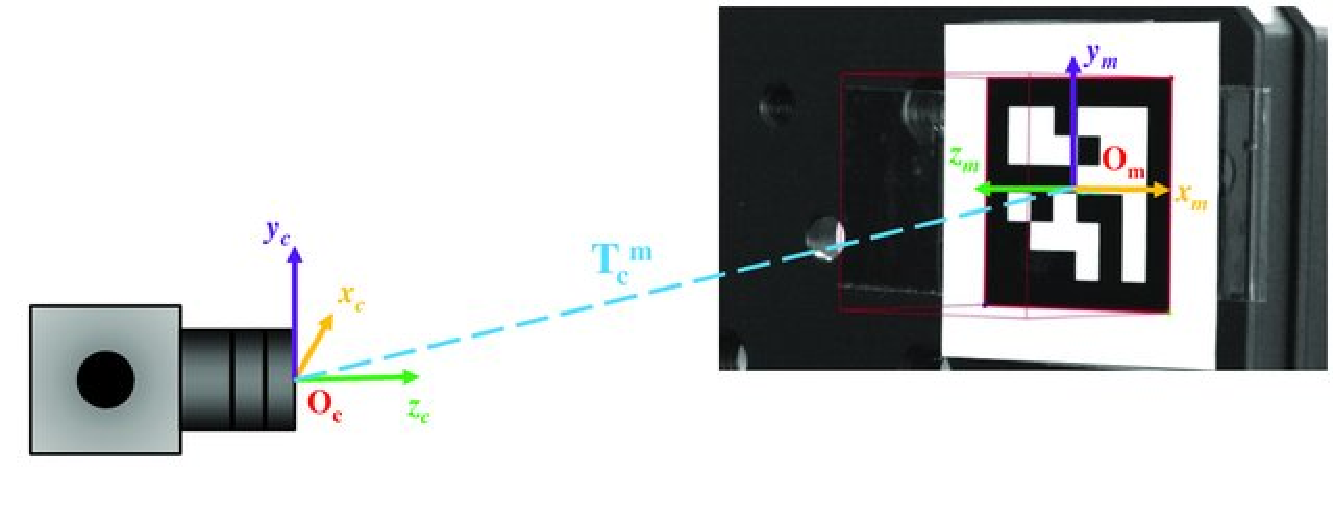
\includegraphics[width=.90\textwidth,angle=0]{figure 3-6.pdf}
    \caption{Súradnicový systém kamery a značky interpretovaný programom OpenCV.}
    \captionsetup{font=footnotesize, justification=centering, skip=5pt}
    \caption*{(Zdroj: Popescu, Dragos. (2018). Automatic rough alignment for key components in laser driven experiments using fiducial markers. Journal of Physics: Conference Series. 1079. 012013. 10.1088/1742-6596/1079/1/012013.)}
    \label{o:3-6}
\end{figure}  
% Popescu, Dragos & Cernaianu, Mihail & Dumitrache, I.. (2018). Automatic rough alignment for key components in laser driven experiments using fiducial markers. Journal of Physics: Conference Series. 1079. 012013. 10.1088/1742-6596/1079/1/012013. 

\subsubsection{Perspektívna projekcia, transformácia pnp}
Perspektívna projekcia je matematická metóda, ktorá sa používa na transformáciu 3D objektov na 2D obrazovú rovinu. Tento vzťah sa nazýva perspektívna projekcia a je založený na princípe podobnosti trojuholníkov. Matematicky môžeme tento proces zapísať ako \citep{9549863}:
\begin{equation}
    \begin{pmatrix} u \\ v \\ 1 \end{pmatrix} =
    \begin{bmatrix}
        f_x & 0 & c_x \\
        0 & f_y & c_y \\
        0 & 0 & 1
    \end{bmatrix}
    \begin{bmatrix}
        r_{11} & r_{12} & r_{13} & t_1 \\
        r_{21} & r_{22} & r_{23} & t_2 \\
        r_{31} & r_{32} & r_{33} & t_3 \\
        0 & 0 & 0 & 1
    \end{bmatrix}
    \begin{bmatrix}
        X \\ 
        Y \\
        Z \\
        1
    \end{bmatrix}
\end{equation}
kde $u$ a $v$ sú pixely v 2D obrazovke, $(X, Y, Z)$ sú súradnice bodu v 3D priestore, $fx$ a $fy$ predstavujú ohniskovú vzdialenosť kamery v osiach $x$ a $y$ v pixely, $cx$ a $cy$ predstavujú súradnice stredu obrazovky v pixely, $r_{11}$ až $r_{33}$ sú prvky rotácie a $t_1$ až $t_3$ predstavujú posun kamery v priestore.

Tento proces zahŕňa vytvorenie modelu kamery, ktorý definuje polohu a orientáciu virtuálnej kamery v 3D priestore. Tento model kamery sa potom použije na premietnutie 3D súradníc objektu do 2D roviny.

Na výpočet transformácie medzi 3D svetovými súradnicami objektu a jeho 2D obrazovými súradnicami sa používa algoritmus PnP (Perspective-n-Point). Túto transformáciu možno použiť na určenie polohy a orientácie objektu v 3D priestore vzhľadom na kameru.

Algoritmus PnP vyžaduje nasledujúce vstupy:
\begin{enumerate}
\item Súbor 3D bodov objektu vyjadrených v súradnicovom systéme vzhľadom na kameru;
\item Súbor 2D obrazových bodov, ktoré zodpovedajú projekcii 3D bodov objektu na 2D obrazovú rovinu;
\item Vlastná matica kamery, ktorá opisuje vnútorné parametre kamery, ako je ohnisková vzdialenosť a hlavný bod;
\item Voliteľne vonkajšia matica kamery, ktorá opisuje polohu a orientáciu kamery v 3D priestore;
\item Algoritmus PnP vypočíta rotáciu a transláciu objektu vzhľadom na kameru pomocou nelineárnej optimalizačnej metódy. Algoritmus minimalizuje chybu reprojekcie, čo je rozdiel medzi projektovanými 3D bodmi a zodpovedajúcimi 2D obrazovými bodmi.
\end{enumerate}

Algoritmus PnP možno riešiť rôznymi metódami vrátane metódy priamej lineárnej transformácie (DLT) a Levenberg-Marquardtovho algoritmu. Metóda DLT zahŕňa riešenie lineárnej sústavy rovníc, zatiaľ čo Levenberg-Marquardtov algoritmus je nelineárna optimalizačná metóda.

Algoritmus PnP je základným nástrojom počítačového videnia a používa sa v mnohých aplikáciách vrátane sledovania objektov, rozšírenej reality a lokalizácie robotov.

Algoritmus PnP je implementovaný vo funkcii OpenCV cv2.solvePnP(), ktorá prijíma vyššie opísané vstupy a vracia vektory rotácie a translácie objektu vzhľadom na kameru. Tieto vektory možno použiť na transformáciu súradníc objektu do súradnicového systému kamery alebo naopak pomocou jednoduchých maticových operácií \citep{opencv_calib3d}.

Vzorec pre transformáciu PnP je nasledujúci:
\begin{equation}
    rvec, tvec = cv2.solvePnP(objectPoints, imagePoints, cameraMatrix, distCoeffs)
\end{equation}
kde:
\begin{enumerate}
\item $\text{objectPoints}$ je pole 3D bodov v súradnicovom systéme objektu;
\item $\text{imagePoints}$ je pole zodpovedajúcich 2D obrazových bodov;
\item $\text{cameraMatrix}$ je vlastná matica kamery;
\item $\text{distCoeffs}$ sú koeficienty skreslenia kamery;
\item $rvec$ je vektor natočenia objektu vzhľadom na kameru;
\item $tvec$ je vektor translácie objektu vzhľadom na kameru.
\end{enumerate}

Vektor rotácie rvec možno previesť na maticu rotácie pomocou funkcie cv2.Rodrigues(). Translačný vektor tvec je vyjadrený v súradnicovom systéme kamery a možno ho použiť na transformáciu súradníc objektu do súradnicového systému kamery pomocou jednoduchej maticovej operácie \citep{opencv_calib3d}:
\begin{equation}
    \textbf{objectPoints}{\textbf{cam}} = \textbf{R} \cdot \textbf{objectPoints}^{\top} + \textbf{t}{\textbf{vec}}
    \end{equation}
Kde $\textbf{objectPoints}{\textbf{cam}}$ je transformované pole 3D bodov objektu v súradnicovom systéme kamery, $\textbf{R}$ je matica rotácie, $\textbf{objectPoints}$ je pole 3D bodov objektu v súradnicovom systéme objektu, $\textbf{t}{\textbf{vec}}$ je vektor translácie objektu vzhľadom na kameru a $\cdot$ predstavuje násobenie matíc.

\subsubsection{Konvencie merania}
Pri riešení problémov počítačového videnia je dôležité stanoviť súbor konvencií merania. Tieto konvencie špecifikujú súradnicový systém používaný na reprezentáciu polôh a orientácií objektov v 3D priestore, ako aj jednotky používané na ich meranie. V tejto časti opíšeme konvencie používané v počítačovom videní, ktoré sú založené na pravotočivom súradnicovom systéme.

\textbf{Pravotočivý súradnicový systém.} Pravotočivý súradnicový systém je najčastejšie používaným systémom v počítačovom videní. Je to trojrozmerný karteziánsky súradnicový systém, v ktorom kladné osi x, y a z smerujú doprava, nahor a k pozorovateľovi. Orientáciu súradnicového systému možno reprezentovať pomocou matice rotácie, ktorá transformuje body zo svetového súradnicového systému do súradnicového systému kamery.

\textbf{Jednotky merania.} Merné jednotky používané v počítačovom videní sú zvyčajne milimetre alebo metre. Tieto jednotky sa používajú na reprezentáciu vzdialeností, napríklad vzdialenosti medzi dvoma bodmi v 3D priestore alebo ohniskovej vzdialenosti kamery. Výber jednotiek závisí od rozsahu riešeného problému.

\textbf{Matica kamery.} Matica kamery je matica 3x4, ktorá predstavuje vnútorné a vonkajšie parametre kamery. Vnútorné parametre opisujú vlastnosti kamery, napríklad ohniskovú vzdialenosť a polohu hlavného bodu, zatiaľ čo vonkajšie parametre opisujú orientáciu a polohu kamery v 3D priestore. Maticu kamery možno zapísať ako:

\begin{equation}
\mathbf{P} = \begin{bmatrix}f_x & 0 & c_x & t_x \\ 0 & f_y & c_y & t_y \\ 0 & 0 & 1 & 0\end{bmatrix},
\end{equation}

kde $f_x$ a $f_y$ sú ohniskové vzdialenosti v smere x a y, $c_x$ a $c_y$ sú súradnice hlavného bodu v obraze a $t_x$ a $t_y$ sú translačné parametre, ktoré opisujú polohu kamery vo svetovom súradnicovom systéme.

\textbf{Projekčná matica.} Projekčná matica je matica 3x4, ktorá mapuje 3D body vo svetovom súradnicovom systéme na 2D body v súradnicovom systéme obrazu. Vypočíta sa ako súčin matice kamery a matice rotácie, ktorá transformuje body zo svetového súradnicového systému do súradnicového systému kamery:

\begin{equation}
\mathbf{P'} = \mathbf{P} \cdot [\mathbf{R} | \mathbf{t}],
\end{equation}
kde $\mathbf{R}$ je matica rotácie a $\mathbf{t}$ je vektor translácie, ktorý opisuje polohu kamery vo svetovom súradnicovom systéme.

\textbf{Homogénny súradnicový systém.} Homogénny súradnicový systém je matematický rámec, ktorý nám umožňuje reprezentovať body v 3D priestore ako 4D vektory. Je to užitočné, pretože nám to umožňuje vykonávať transformácie, ako je translácia a rotácia, pomocou násobenia matíc. 3D bod $\mathbf{X} = [X, Y, Z]$ vo svetovom súradnicovom systéme možno reprezentovať v homogénnych súradniciach ako $\mathbf{X}_h = [X, Y, Z, 1]$. Podobne bod $\mathbf{x} = [u, v]$ v súradnicovom systéme obrazu možno reprezentovať v homogénnych súradniciach ako $\mathbf{x}_h = [u, v, 1]$.

Keďže neexistuje všeobecná dohoda o konvencii pre Eulerove uhly, musíme definovať používanú konvenciu. V tomto prípade ukladáme uhly v už spomínanom poradí podľa záporných hodnôt získaných z dronu SDK. Tie sú totožné s konvenciou uhlov používanou pre lietadlá podľa letovej normy DIN 9300-2 (obrázok 3-6). Presnejšou definičnou skupinou pre konvenciu vybraných uhlov je vlastná konvencia Tait-Bryanových uhlov z-y'-x", známa aj ako námorné alebo Cardanove uhly \citep{DIN9300-2}.
\begin{figure}[ht!]
    \centering
    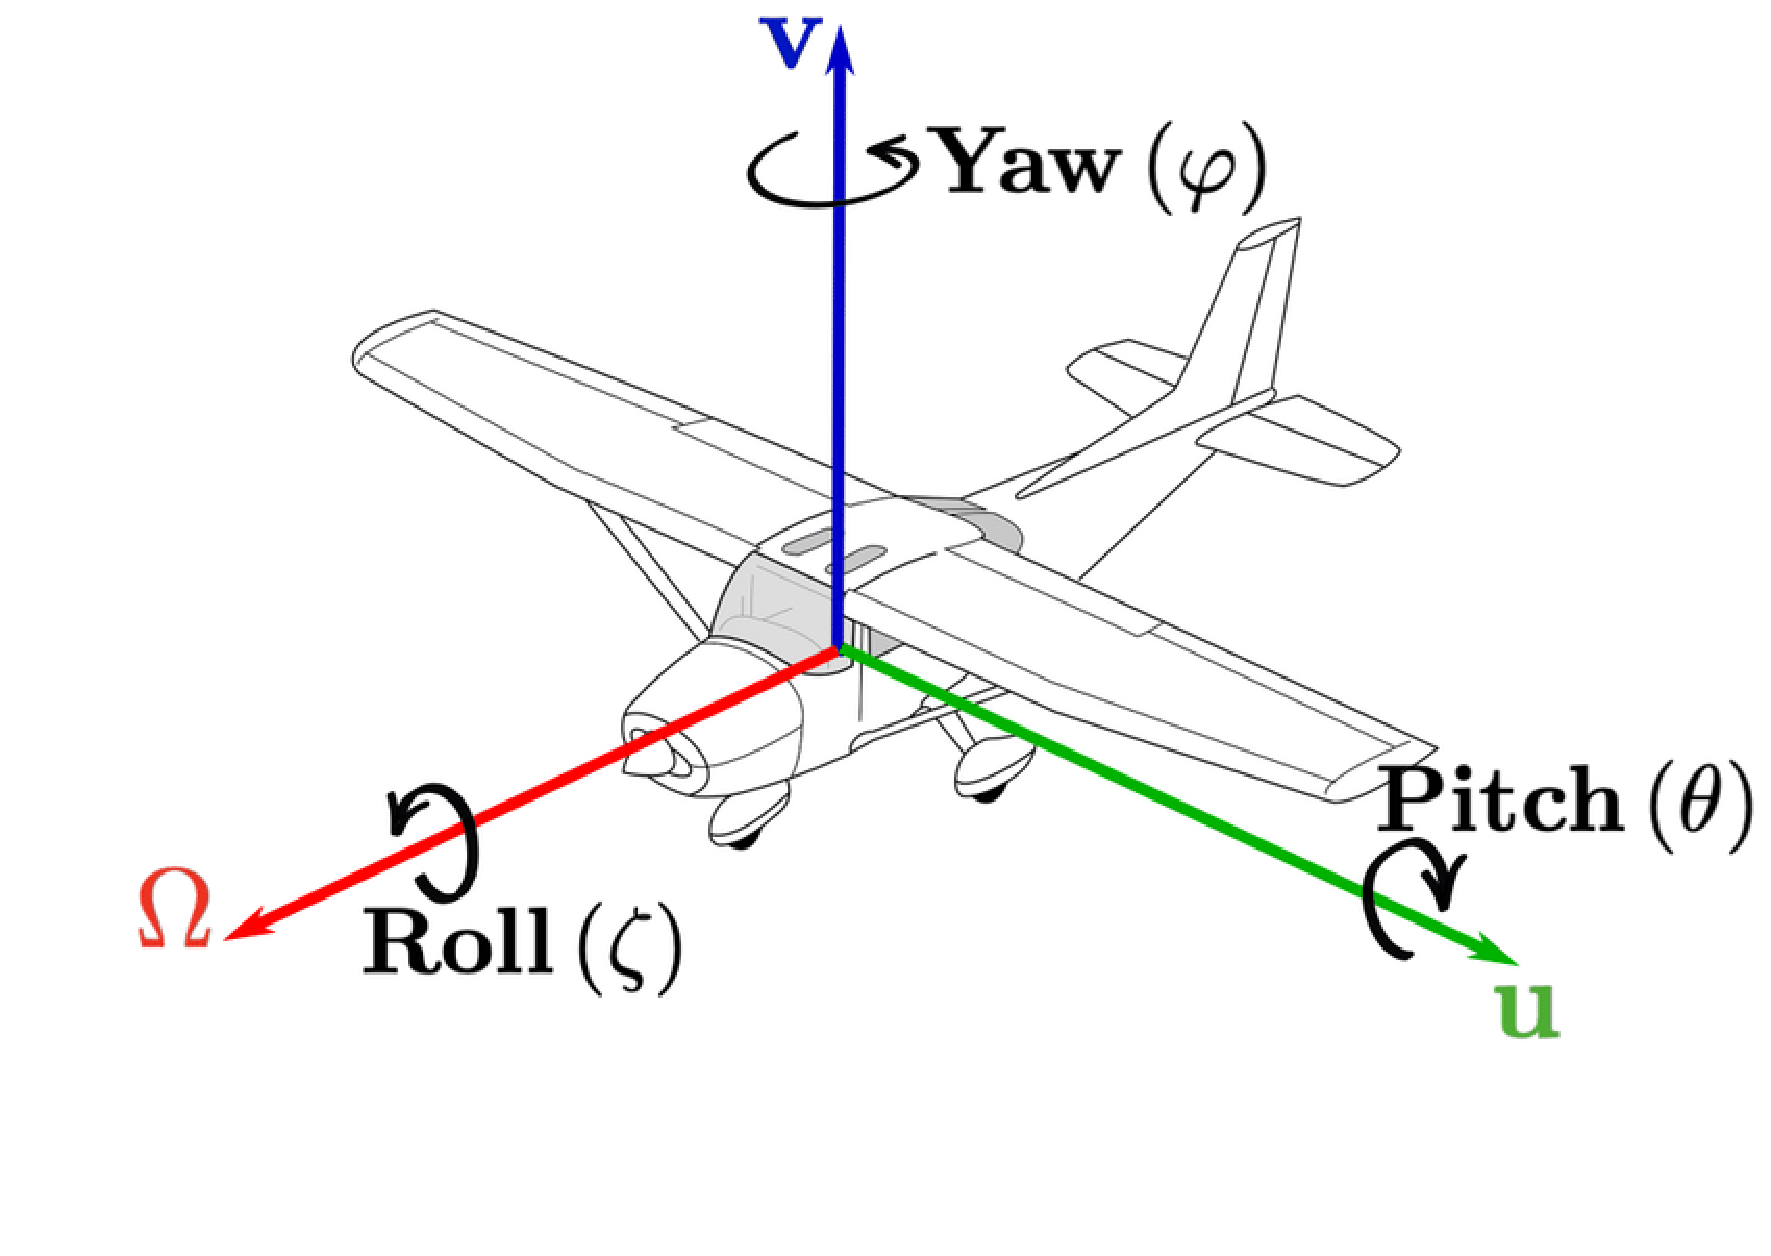
\includegraphics[width=.65\textwidth,angle=0]{figure 3-8.pdf}
    \caption{Hlavné nápravy lietadla podľa normy DIN 9300.}
    \captionsetup{font=footnotesize, justification=centering, skip=5pt}
    \caption*{(Zdroj: vlastné spracovanie)}
    \label{o:3-8} 
\end{figure} 

\subsubsection{Konvencie používané v opencv}
OpenCV používa špecifický súbor konvencií na reprezentáciu bodov, rotácií a translácií \citep{opencv_calib3d}. Tieto konvencie je dôležité pochopiť pri práci s knižnicou. Tu sú niektoré z hlavných konvencií používaných v OpenCV:

Body sú reprezentované ako súradnice (x, y) s počiatkom (0, 0) v ľavom hornom rohu obrazu.

Rotácie sú reprezentované pomocou Rodriguesovho rotačného vzorca, ktorý konvertuje 3D rotačný vektor na 3x3 rotačnú maticu. Vektor rotácie je definovaný ako (rx, ry, rz), kde rx, ry a rz predstavujú uhly rotácie okolo osí x, y a z.

Translácie sú reprezentované ako 3D vektory (tx, ty, tz).

Vlastné parametre kamery sú reprezentované pomocou nasledujúcej matice:
\begin{equation}
\begin{bmatrix}
f_x & 0 & c_x \\
0 & f_y & c_y \\
0 & 0 & 1
\end{bmatrix}
\end{equation}

kde fx a fy sú ohniskové vzdialenosti kamery v smere x a y a cx a cy sú súradnice hlavného bodu (bod, v ktorom optická os pretína rovinu obrazu).

Vonkajšie parametre kamery sú reprezentované pomocou matice 3x4, ktorá kombinuje rotáciu a transláciu:
\begin{equation}
\begin{bmatrix}
r_{11} & r_{12} & r_{13} & t_x \\
r_{21} & r_{22} & r_{23} & t_y \\
r_{31} & r_{32} & r_{33} & t_z
\end{bmatrix}
\end{equation}
kde ľavý horný stĺpec matice 3x3 predstavuje maticu rotácie a pravý stĺpec predstavuje vektor translácie.

Medzi hodnotami vrátenými funkciou estimatePoseSingleMarkers() sa vektor translácie interpretuje v metroch a vektor rotácie používa reprezentáciu osového uhla alebo Rodriguesovu reprezentáciu, čo je najkompaktnejšia forma uloženia matice rotácie. Funkcia Rodrigues() v OpenCV dokáže vypočítať maticu rotácie z vektorov rotácie zadaných ako riadkové vektory podľa rovnice (3.8.) a dokáže určiť aj jej inverziu, ak je vstupom matica rotácie.
\begin{figure}[ht!]
    \centering
    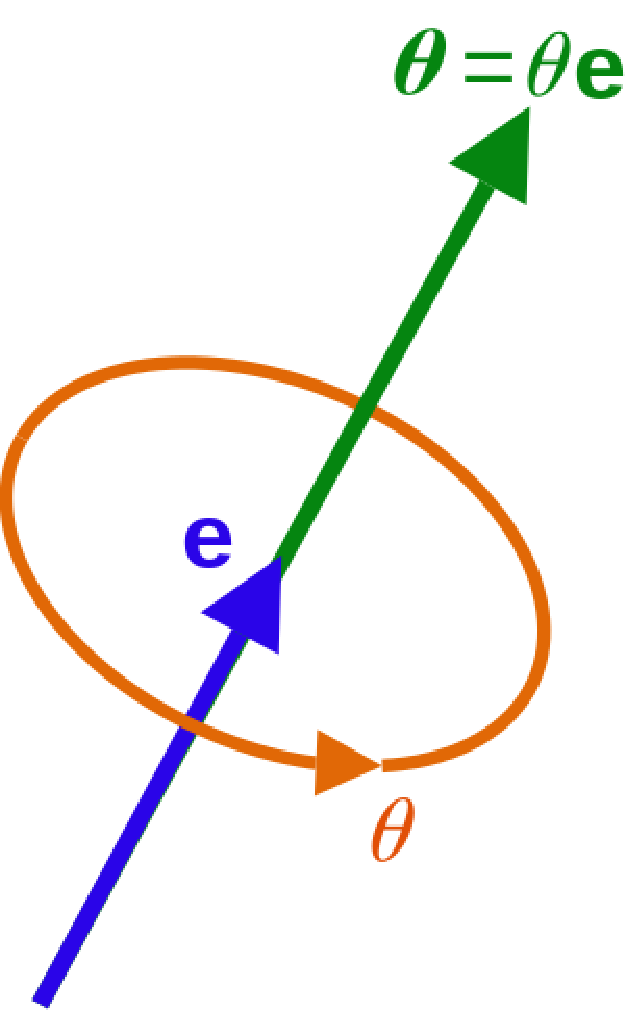
\includegraphics[width=.13\textwidth,angle=0]{figure 3-7.pdf}
    \caption{Interpretácia vektora natočenia Rodriguesovej osi a uhla.}
    \label{o:3-7} 
\end{figure}
% https://en.wikipedia.org/wiki/Axis%E2%80%93angle_representation

\subsubsection{Prevod polohy kamery do globálneho súradnicového systému}
Na prevod polohy kamery (ktorá sa nachádza v počiatku súradnicového systému kamery) do globálneho súradnicového systému musíme použiť vektory rotácie a translácie získané z funkcie solvePnP v OpenCV.

Vektor rotácie (rvec) udáva rotáciu súradnicového systému kamery vzhľadom na súradnicový systém značky a vektor translácie (tvec) udáva polohu značky v súradnicovom systéme kamery.

Na prevod polohy kamery do globálneho súradnicového systému musíme postupovať podľa týchto krokov:

\textbf{1. Vypočítame maticu rotácie R} z vektora rotácie rvec pomocou Rodriguesovho vzorca:
\begin{equation}
R = \begin{bmatrix}
\cos\theta + u_x^2(1-\cos\theta) & u_x u_y (1-\cos\theta) - u_z \sin\theta & u_x u_z (1-\cos\theta) + u_y \sin\theta \\
u_y u_x (1-\cos\theta) + u_z \sin\theta & \cos\theta + u_y^2(1-\cos\theta) & u_y u_z (1-\cos\theta) - u_x \sin\theta \\
u_z u_x (1-\cos\theta) - u_y \sin\theta & u_z u_y (1-\cos\theta) + u_x \sin\theta & \cos\theta + u_z^2(1-\cos\theta) \\
\end{bmatrix}
\end{equation}

kde $\theta$ je veľkosť vektora rotácie a $u_x$, $u_y$ a $u_z$ sú zložky jednotkového vektora v smere vektora rotácie.

\textbf{2. Vypočítame inverznú hodnotu matice rotácie R}, ktorá predstavuje rotáciu súradnicového systému značky vzhľadom na súradnicový systém kamery.

\textbf{3. Vypočítame inverzný vektor translácie tvec}, ktorý predstavuje polohu kamery v súradnicovom systéme značky.

\textbf{4. Vypočítame súčin inverznej matice rotácie} a inverzného translačného vektora:

\begin{equation}
-R^{-1}t_{vec}
\end{equation}

Takto získame polohu kamery v súradnicovom systéme značky.

\textbf{5. Preveďme polohu kamery} v súradnicovom systéme značky do globálneho súradnicového systému pripočítaním polohy značky v globálnom súradnicovom systéme:
\begin{equation}
P_{global} = P_{značka} + R_{značka}^{-1}(-R^{-1}t_{vec})
\end{equation}

kde $P_{značka}$ je poloha značky v globálnom súradnicovom systéme a $R_{marker}$ je rotačná matica, ktorá definuje orientáciu značky v globálnom súradnicovom systéme.

Výsledný vektor $P_{global}$ je poloha kamery v globálnom súradnicovom systéme.

V súhrne sú kroky na prevod polohy kamery do globálneho súradnicového systému nasledovné:

Výpočet matice rotácie R z vektora rotácie rvec pomocou Rodriguesovho vzorca.
Výpočet inverznej matice rotácie R na získanie matice rotácie reprezentujúcej súradnicový systém značky vzhľadom na súradnicový systém kamery.
Vypočítame inverzný vektor translácie tvec


\subsection{Webové sokety s komunikáciou s dronom}
Webové sokety sú populárnym mechanizmom na komunikáciu v reálnom čase medzi klientom a serverom cez web. V kontexte riadenia dronov sa webové sokety môžu použiť na vytvorenie trvalého obojsmerného kanála medzi pozemnou stanicou (klientom) a dronom (serverom), ktorý umožňuje výmenu príkazov, telemetrických údajov a videoprenosov v reálnom čase.

\begin{figure}[ht!]
    \centering
    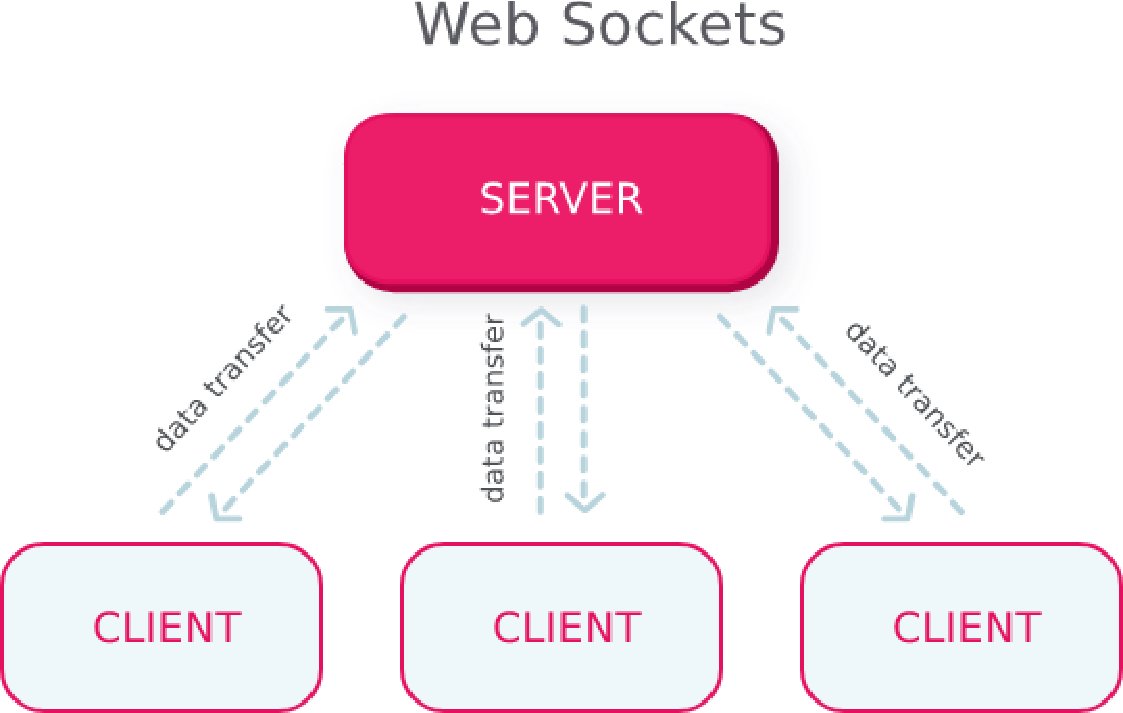
\includegraphics[width=.70\textwidth,angle=0]{figure 3-9.pdf}
    \caption{Štandardný režim fungovania webových soketov.}
    \captionsetup{font=footnotesize, justification=centering, skip=5pt}
    \caption*{(Zdroj: vlastné spracovanie)}
    \label{o:3-9}
\end{figure}  

\subsubsection{Architektúra}
Typická architektúra komunikačného systému dronu založeného na webových zásuvkách pozostáva z troch hlavných komponentov: pozemnej stanice, dronu a web-socket servera. Pozemná stanica je zodpovedná za generovanie používateľských príkazov a prijímanie telemetrických údajov a video prúdov z dronu. Dron je zodpovedný za vykonávanie príkazov a zachytávanie telemetrických údajov a video prúdov. Webový socketový server funguje ako middleware medzi pozemnou stanicou a dronom, spracováva komunikačný protokol a preposiela správy v reálnom čase (obrázok 3-9).



\subsubsection{Komunikačný protokol}
Komunikačný protokol pre systém dronu založený na webo-socket pozostáva z dvoch typov správ: príkazových správ a telemetrických správ.

\textbf{Príkazové správy.} Príkazové správy sa posielajú z pozemnej stanice do dronu a pozostávajú z pokynov pre dron, aby vykonal určitú činnosť, napríklad vzlietol, pristál, pohol sa dopredu alebo odbočil doľava. Formát príkazových správ sa môže líšiť v závislosti od modelu dronu a špecifických funkcií, ktoré sa používajú, ale bežný formát je JSON (JavaScript Object Notation). Napríklad príkazová správa o vzlete vo formáte JSON môže vyzerať takto:
\begin{verbatim}
{
  "command": "takeoff",
  "args": []
}
\end{verbatim}

\textbf{Telemetrické správy.} Príkazové správy sa posielajú z pozemnej stanice do dronu a pozostávajú z pokynov pre dron, aby vykonal určitú činnosť, napríklad vzlietol, pristál, pohol sa dopredu alebo odbočil doľava. Formát príkazových správ sa môže líšiť v závislosti od modelu dronu a špecifických funkcií, ktoré sa pTelemetrické správy sa odosielajú z dronu do pozemnej stanice a pozostávajú z údajov snímačov, ako sú súradnice GPS, nadmorská výška, úroveň nabitia batérie a údaje z kamery. Formát telemetrických správ sa môže líšiť aj v závislosti od modelu dronu a konkrétnych použitých snímačov, ale JSON je opäť bežný formát. Napríklad telemetrická správa Tello drona o svojom $state$ vo formáte JSON môže vyzerať takto:
\begin{verbatim}
    {
        "pitch": 0,
        "roll": 0,
        "yaw": 0,
        "vgx": 0,
        "vgy": 0,
        "vgz": 0,
        "templ": 62,
        "temph": 65,
        "tof": 10,
        "h": 0,
        "bat": 58,
        "baro": 40.39,
        "time": 0,
        "agx": 7.00,
        "agy": 19.00,
        "agz": -999.00
      }
\end{verbatim}
Tento objekt obsahuje rôzne informácie o stave dronu vrátane uhlov náklonu, natočenia a vychýlenia, rýchlosti pozdĺž osí x, y a z, teploty, vzdialenosti počas letu, úrovne nabitia batérie, barometrického tlaku a zrýchlenia pozdĺž osí x, y a z.

\subsubsection{Implementácia}
Na implementáciu komunikačného systému dronu založeného na web-sockets možno postupovať podľa nasledujúcich krokov:
\begin{itemize}
    \item Nastaviť web-socket server, ktorý dokáže spracovať prichádzajúce spojenia z pozemnej stanice a dronu a preposielať správy medzi nimi.
    \item Implementovať skript na strane klienta na pozemnej stanici, ktorý dokáže nadviazať spojenie webového socketu so serverom, odosielať príkazové správy do dronu a prijímať telemetrické správy z dronu.
    \item Implementovať skript na strane servera na dron, ktorý môže vytvoriť spojenie webového socketu so serverom, prijímať príkazové správy z pozemnej stanice a posielať telemetrické správy pozemnej stanici.
    \item Integrovať skripty na strane klienta a servera s riadiacim softvérom dronu a používateľským rozhraním na pozemnej stanici.
\end{itemize}

%   
% !TeX encoding = UTF-8
% !TeX spellcheck = sk_SK
% !TeX root=tukedip.tex

\section{Implementácia projektu}
V tejto časti podrobne opíšeme realizáciu nášho projektu. Opíšeme architektúru systému a účel jednotlivých modulov. Poskytneme aj prehľad štruktúry kódu a funkčnosti jednotlivých súborov. Okrem toho vysvetlíme, ako sme do nášho projektu integrovali rôzne technológie a knižnice, aby sme dosiahli naše ciele. Nakoniec rozoberieme všetky problémy, s ktorými sme sa stretli počas procesu implementácie, a ako sme ich riešili.
\subsection{Prehľad štruktúry programov} 

    \begin{center}
        \begin{tikzpicture}[node distance=3cm]
            \node (main) [draw, rectangle] {main.py};
            \node (tello) [draw, rectangle, below of=main] {tello.py};
            \node (cam) [draw, rectangle, right of=main, xshift=2cm] {cam\_class.py};
            \node (targeter) [draw, rectangle, right of=cam, xshift=2cm] {targeter.py};
            \node (video) [draw, rectangle, below of=tello] {video\_writer.py};
            \node (marker) [draw, rectangle, below of=cam] {marker\_class.py};
            \node (pid) [draw, rectangle, below of=targeter] {pid.py};
            \node (transform) [draw, rectangle, below of=marker] {transformations.py};

            \draw[-latex] (main) -- (tello);
            \draw[-latex] (tello) -- (main);
            \draw[-latex] (main) -- (cam);
            \draw[-latex] (cam) -- (main);
            \draw[-latex] (cam) -- (targeter);
            \draw[-latex] (targeter) -- (cam);
            \draw[-latex] (targeter) -- (pid);
            \draw[-latex] (pid) -- (targeter);
            \draw[-latex] (tello) -- (video);
            \draw[-latex] (cam) -- (marker);
            \draw[-latex] (marker) -- (transform);
            \draw[-latex] (transform) -- (marker);
        \end{tikzpicture}
    \end{center}

    \textbf{Popis:}

    \textbf{main.py} - Obsahuje grafické rozhranie pyGame a zobrazenie obrazu kamery. Používa rôzne klávesy na klávesnici na prepínanie funkcií alebo ovládanie dronu.

    \textbf{tello.py} - Obsahuje funkcie na komunikáciu s dronom a čítanie údajov.

    \textbf{video\_writer.py} - Beží na samostatnom vlákne, zachytáva video počas automatického ovládania a potom ho vypúšťa.

    \textbf{cam\_class.py} - Vykonáva úlohy spracovania obrazu (kalibrácia, rozpoznávanie značiek) a údaje o rýchlosti dronu sa odtiaľto zaraďujú do frontu. Odovzdáva načítané pozície značiek funkciám, ktoré ich spracúvajú.

    \textbf{targeter.py} - Prečíta funkcie zodpovedajúce poradovým číslam značiek zo zadaného súboru CSV a vráti vektor kontrolnej základne.

    \textbf{pid.py} - Obsahuje triedu implementujúcu numerický PID regulátor, vypočítava hodnoty regulačného stupňa.

    \textbf{marker\_class.py} - Trieda, ktorá uchováva všetky údaje pre značky. Počas zberu údajov počíta a nakoniec zapisuje zozbierané pozície do súboru NPZ.
 
    \textbf{transformations.py} - Implementuje transformácie súradnicového systému a obsahuje funkcie na konverziu vektorov rotácie.

 
\subsection{Ovládanie drona}
Dron Tello sa ovláda pomocou kombinácie softvérových programov, ktoré s ním komunikujú prostredníctvom pripojenia Wi-Fi (obrázok 4-1). Na nízkoúrovňovú komunikáciu medzi dronom a riadiacim počítačom sa používa knižnica Tello Python, tello.py.

\begin{figure}[ht!]
    \centering
    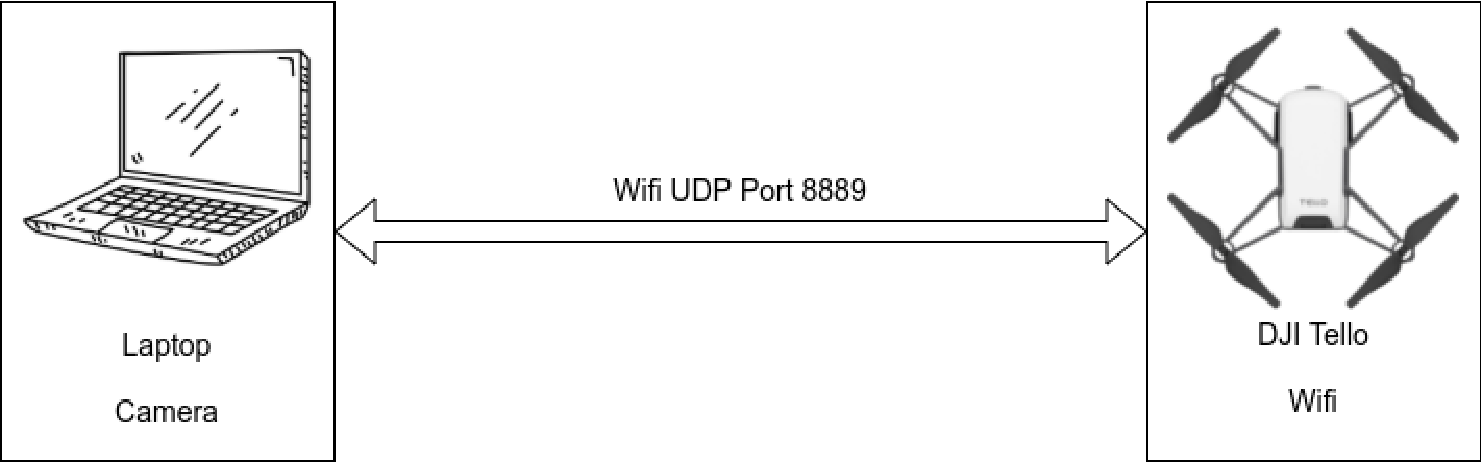
\includegraphics[width=.70\textwidth,angle=0]{figure 4-3.pdf}
    \caption{Schéma procesu pripojenia dronu.}
    \captionsetup{font=footnotesize, justification=centering, skip=5pt}
    \caption*{(Zdroj: vlastné spracovanie)}
    \label{o:4-3} 
\end{figure}  

Knižnica tello.py poskytuje množstvo funkcií, ktoré možno použiť na odosielanie príkazov do dronu a prijímanie údajov z neho. Medzi tieto funkcie patria 
$takeoff()$, $land()$, $move\_left()$, $move\_right()$, $move\_forward()$, $move\_backward()$, \break $rotate\_clockwise()$, $rotate\_counter\_clockwise()$ 
a mnohé ďalšie. Knižnica obsahuje aj funkcie na získavanie údajov z dronu, ako je jeho aktuálna výška, úroveň nabitia batérie a čas letu.

Na ovládanie dronu Tello z webovej aplikácie program využíva spojenie "web-sockets" na komunikáciu so skriptom Python na strane servera. Tento skript funguje ako most medzi webovou aplikáciou a dronom Tello a prenáša medzi nimi príkazy a údaje.

Skript na strane servera používa knižnicu tello.py na odosielanie príkazov do dronu a prijímanie údajov z neho. Keď používateľ zadá príkaz vo webovej aplikácii, príkaz sa odošle na server prostredníctvom spojenia "web-sockets". Server potom použije príslušnú funkciu v knižnici tello.py na odoslanie príkazu dronu. Po vykonaní príkazu môže server získať všetky relevantné údaje z dronu a poslať ich späť do webovej aplikácie na zobrazenie.

Celkovo kombinácia tello.py a skriptu na strane servera poskytuje výkonnú platformu na ovládanie dronu Tello z webovej aplikácie. Vďaka možnosti odosielať širokú škálu príkazov a získavať podrobné údaje z dronu.

\subsection{Spracovanie obrázkov}
S riadením dronov úzko súvisí, ale viac sa zaoberá spracovaním obrazu, program cam\_class.py, ktorého hlavná funkcia je zodpovedná za rozpoznávanie značiek ArUco. ArUco značky sa zisťujú pomocou vstavanej funkcie OpenCV cv2.aruco.detectMarkers(). Tá nájde kódy v načítanom zväzku značiek po adaptívnej segmentácii aplikovanej na obraz v odtieňoch sivej a vráti ich rohové body v pixeloch a ich poradové číslo. Na výpočet skutočnej trojrozmernej polohy značiek na základe matíc kamery sa používa už spomínaná transformácia PnP. Výsledné polohy s ich poradovým číslom značky sa môžu odoslať na ďalšie spracovanie (časť 4.4) alebo použiť na automatickú navigáciu dronu.

Program je určený na navigáciu dronu Tello pomocou značiek umiestnených na zemi. To sa dosiahne použitím knižnice OpenCV na detekciu značiek vo videozázname z kamery dronu.
\begin{mypython}[caption={Inicializácia parametrov detekcie značiek OpenCV},label=CL-3]

    import cv2
    import numpy as np
    from djitellopy import Tello
    
    # Initialize Tello drone
    tello = Tello()
    tello.connect()
    tello.streamon()
    
    # Initialize OpenCV marker detection parameters
    aruco_dict = cv2.aruco.Dictionary_get(cv2.aruco.DICT_6X6_250)
    aruco_params = cv2.aruco.DetectorParameters_create()
    
    # Set up video stream
    stream = tello.get_video_stream()
\end{mypython}

Program najprv inicializuje kameru a nastaví tok videa. Potom pomocou slučky nepretržite zachytáva snímky z videoprenosu a spracováva ich. Pre každú snímku program používa vstavané funkcie OpenCV na detekciu značiek a odhad ich polohy v 3D priestore.
\begin{mypython}[caption={Detekcia značky a vypočítanie polohy},label=CL-4]
    while True:
    # Capture frame from video stream
    frame = stream.read()

    # Detect markers in frame
    corners, ids, rejected = cv2.aruco.detectMarkers(frame, aruco_dict, parameters=aruco_params)

    # Estimate marker position in 3D space
    rvecs, tvecs, _ = cv2.aruco.estimatePoseSingleMarkers(corners, 0.05, camera_matrix, dist_coeffs)

    # Process marker positions
    if ids is not None:
        # TODO: Implement control algorithm
        pass

    # Display frame
    cv2.imshow('Frame', frame)
    if cv2.waitKey(1) & 0xFF == ord('q'):
        break

\end{mypython}

Po odhadnutí polohy značiek program pomocou proporcionálneho riadiaceho algoritmu upravuje odklon, sklon a výšku dronu na základe polohy značiek vzhľadom na stred snímky. Algoritmus vypočíta chybu medzi stredom rámu a polohou značiek a upraví orientáciu a výšku dronu tak, aby sa táto chyba minimalizovala.

Program obsahuje aj niekoľko bezpečnostných funkcií, ktoré zabraňujú kolízii dronu s prekážkami alebo vyleteniu mimo dosahu. Medzi tieto funkcie patrí nastavenie maximálnej výšky a doletu dronu, ako aj detekcia prekážok v dráhe dronu a automatické nastavenie jeho trajektórie tak, aby sa im vyhol.

Na ďalšie zlepšenie presnosti a spoľahlivosti detekcie a sledovania značiek program obsahuje množstvo konfigurovateľných parametrov, ako je minimálna a maximálna veľkosť značky, prah detekcie a proporcionálne zisky riadenia. Tieto parametre sa dajú upraviť tak, aby sa optimalizoval výkon programu pre rôzne prostredia a svetelné podmienky.

Celkovo program poskytuje spoľahlivý a efektívny spôsob navigácie dronu Tello pomocou značkovačov. Použitím knižnice OpenCV na detekciu a sledovanie značiek v reálnom čase a implementáciou proporcionálneho riadiaceho algoritmu na úpravu orientácie a výšky dronu je program schopný navigovať dron s vysokou mierou presnosti a precíznosti.

\subsection{Spracovanie údajov}
Spracovanie priestorových bodov a rotácií získaných z programov na spracovanie obrazu z kamery, t. j. zber údajov, vykonáva program marker\_class.py. Potrebné transformácie, ktoré sú opísané vyššie, vykonávajú funkcie transformations.py.
\subsubsection{Ukladanie údajov o značkách}
Na spracovanie sa môžu odovzdať len údaje značiek, ktoré nemajú žiadny zo svojich vrcholov v pixelovom rámci obrazu. Definícia hrany je 2-2-2-2 \% priesečník na všetkých štyroch stranách obrazu kamery. Značkovače umiestnené na okrajoch poskytujú po odstránení skreslenia jednak nepresnejšie údaje, jednak môžu spôsobiť neistotu označenia vonkajších okrajov 2D kódu značkovača počas detekcie značkovača, ako je to vidieť na obrázku 20.
%TODO: obrazok

V triede markers sú vlastnosti značiek, ktoré ste doteraz videli, uložené v rôznych zoznamoch, ako napríklad:
\begin{itemize}
    \item \textbf{ids}: počet už použitých značiek
    \item \textbf{tvec\_origin}: "markerorigos" v globálnom súradnicovom systéme
    \item \textbf{rvec\_origin}: otočenie súradnicového systému značiek vzhľadom na globálny
    \item \textbf{dRot}: matica rotácie od danéj značky ku globálnemu.
    \item \textbf{allow\_use}: pomocná premenná, ktorá umožňuje použitie danéj značky pri priemerovaní, akonáhle sa zozbiera dostatočný počet vzoriek, môže sa započítať
    \item \textbf{tvec\_min, tvec\_max}: pomocné premenné na filtrovanie výpočtu priemeru
\end{itemize}

Funkcia appendMarker() volaná počas detekcie značiek ArUco pridá nové značky do triedy značiek. Za počiatok berie značku s číslom 1 a na základe jej Eulerovho uhlového natočenia okolo osi x určí, či ide o horizontálnu alebo vertikálnu značku. Ukladá tiež základné hodnoty uhlových rotácií z čítania stavov dronu, to sa stáva počiatkom Eulerových uhlov. Ukladá príslušnú jednu z dvoch orientácií do matice, ktorá bude relevantná pre indexovanie po spracovaní invertovaním smerov vektora translácie.

Ďalšie značky sa ukladajú vytvorením transformácií medzi súradnicovými systémami, ktoré sú implementované skriptom getTransformations() v súbore transformations.py. V prevádzke systém v súčasnosti pracuje s 12 platnými vzormi. Testy boli vykonané s vyššími limitmi platnosti, ale mnohokrát systém nestihol vykonať transformácie, kým sa značky nenachádzali v zornom poli dronu a nebol schopný vypočítať ďalšie. Preto sa zozbiera 12 vektorov posunu medzi dvoma značkami, pričom sa vyradia minimálne a maximálne normály a z 10 zostávajúcich hodnôt sa vytvorí priemer. Matice natočenia sa tiež získajú spriemerovaním 12 vzoriek bez filtrovania. Výsledné hodnoty sa uložia do zoznamov objektov triedy.

Ak už má značka vzorku na autorizáciu, možno ju spočítať pomocou funkcie v úryvku kódu 5. Program spočíta pozície načítané zo všetkých pozorovaných značiek, spriemeruje ich a uloží túto hodnotu pozície. Od uhlových natočení načítaných zo snímača dronu odpočíta počiatok uhlov, čím získa orientáciu dronu.
    % """
    % Calculates the position of the camera relative to the marker, given the marker position and orientation,
    % and the camera position and orientation.
    % Arguments:
    % - marker_pos: A numpy array representing the position of the marker in 3D space.
    % - marker_orient: A numpy array representing the orientation of the marker in 3D space.
    % - camera_pos: A numpy array representing the position of the camera in 3D space.
    % - camera_orient: A numpy array representing the orientation of the camera in 3D space.
    % Returns:
    % - A numpy array representing the position of the camera relative to the marker in 3D space.
    % """
\begin{mypython}[caption={Vypočíta polohu kamery vzhľadom na značku},label=CL-4]
    def calculate_position(marker_pos, marker_orient, camera_pos, camera_orient):
    # rotation matrix for the marker orientation
    marker_rot = cv2.Rodrigues(marker_orient)[0]
    # rotation matrix for the camera orientation
    camera_rot = cv2.Rodrigues(camera_orient)[0]
    # transformation matrix from marker to camera coordinates
    marker_to_camera = np.hstack((marker_rot.T, -marker_rot.T.dot(marker_pos.reshape(3,1))))
    # transformation matrix from camera to global coordinates
    camera_to_global = np.hstack((camera_rot, camera_pos.reshape(3,1)))
    # transformation matrix from marker to global coordinates
    marker_to_global = camera_to_global.dot(marker_to_camera)
    # position of the camera relative to the marker
    camera_rel_marker = marker_to_global[:,3]
    
    return camera_rel_marker
\end{mypython}
\subsection{Webová aplikácia}
Vývoj webovej aplikácie je základnou súčasťou riadiaceho systému pre viacero dronov Tello. Táto webová aplikácia slúži ako používateľské rozhranie na ovládanie dronov v individuálnom aj skupinovom režime. S cieľom zabezpečiť bezproblémové a používateľsky prívetivé prostredie je webová aplikácia navrhnutá s moderným a intuitívnym rozhraním s využitím najnovších technológií vývoja webových aplikácií.

Webová aplikácia je rozdelená na dve hlavné zložky: frontend a backend(obrázok 4-2). Frontend je zodpovedný za prezentáciu používateľského rozhrania a obsluhu interakcie používateľa, zatiaľ čo backend zabezpečuje komunikáciu medzi webovou aplikáciou a dronmi.

\begin{figure}[ht!]
    \centering
    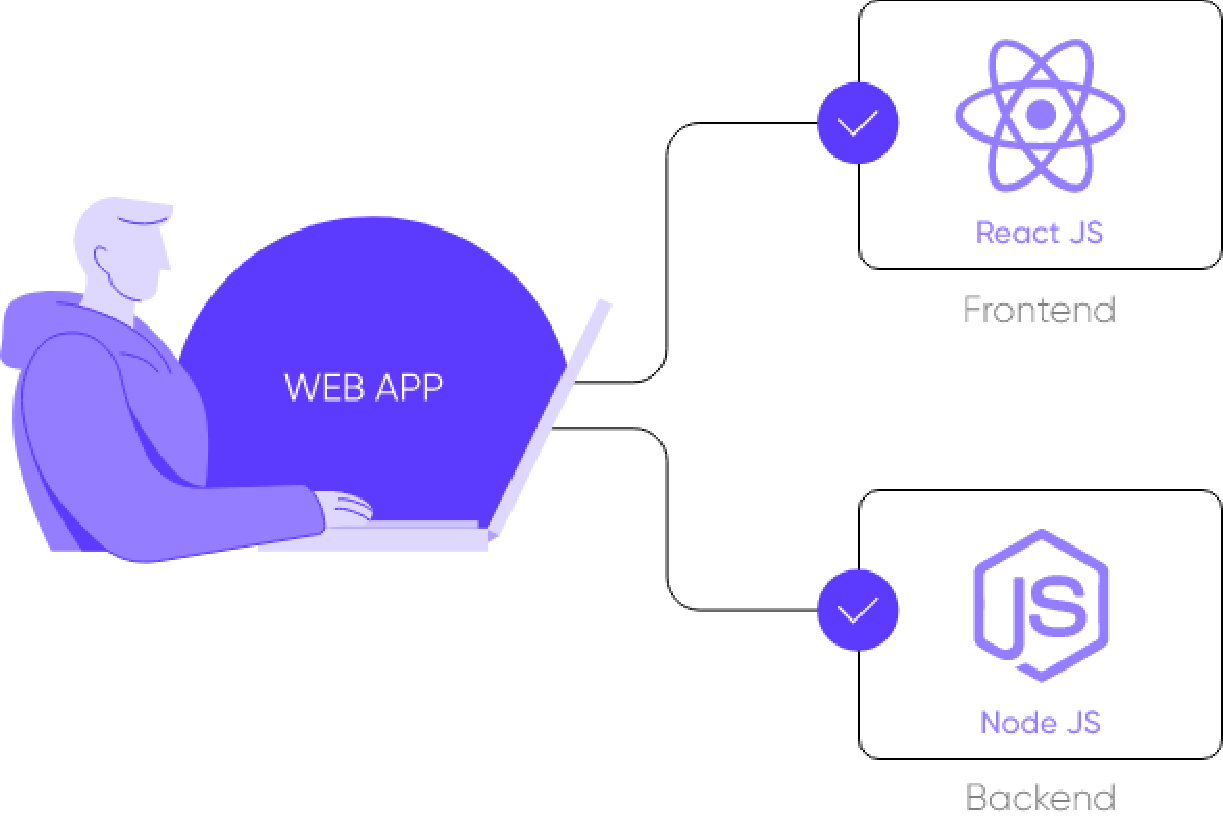
\includegraphics[width=.50\textwidth,angle=0]{figure 4-2.pdf}
    \caption{Schéma rozdelenia webovej aplikácie.}
    \captionsetup{font=footnotesize, justification=centering, skip=5pt}
    \caption*{(Zdroj: vlastné spracovanie)}
    \label{o:4-2}
\end{figure}  

\subsubsection{Frontend}
Webová aplikácia React sa skladá z viacerých komponentov, ktoré spolupracujú pri ovládaní dronov. Keď sa používateľ prihlási do aplikácie, zobrazí sa mu ovládací panel, na ktorom sú zobrazené dostupné drony a ich stav. Informačný panel sa aktualizuje v reálnom čase pomocou webových soketov, aby odrážal zmeny stavu dronov.

Komponent ovládania dronov umožňuje používateľovi vybrať dron a ovládať jeho pohyb pomocou virtuálneho joysticku. Komponent joystick je vytvorený pomocou vlastného rozhrania joysticku. Keď používateľ pohybuje joystickom, komponent posiela príkazy do letového ovládača dronu prostredníctvom webových soketov. Pohyb dronu sa aktualizuje v reálnom čase.

Komponent telemetrie dronu poskytuje v reálnom čase spätnú väzbu o stave dronu vrátane jeho výšky, úrovne nabitia batérie a polohy GPS. Komponent prijíma telemetrické údaje z letového ovládača dronu prostredníctvom pripojenia WebSocket a aktualizuje prístrojový panel s najnovšími informáciami.

Funkčný komponent React, ktorý slúži ako hlavný vstupný bod aplikácie, používa háčik useState na správu stavu rôznych premenných, ktoré určujú aktuálny stav dronu, napríklad jeho nadmorskú výšku, rýchlosť a úroveň batérie. Háčik useEffect sa používa na vykonávanie vedľajších efektov, ako je prihlásenie sa k udalostiam zo servera WebSocket, aktualizácia používateľského rozhrania v reakcii na zmeny stavu a vyčistenie zdrojov, keď je komponent odpojený.

Háčik useContext sa používa na zdieľanie stavu a funkcií medzi rôznymi komponentmi aplikácie. To umožňuje vytvoriť modulárnejšiu a udržiavateľnejšiu kódovú základňu, pretože každá zložka musí vedieť len o stave a funkciách, ktoré sú relevantné pre jej funkčnosť.

Komponenty Material UI, ktoré sa v aplikácii používajú, poskytujú konzistentné a vizuálne príťažlivé používateľské rozhranie. Mriežka sa používa na responzívne a flexibilné rozloženie rôznych komponentov, zatiaľ čo ToggleButton, Tabs, Tab, Button, Typography a Box sa používajú na poskytovanie tlačidiel, štítkov a iných prvkov používateľského rozhrania.

Vlastná komponenta BatteryGauge sa používa na zobrazenie aktuálnej úrovne nabitia batérie dronu vizuálne príťažlivým a zrozumiteľným spôsobom. Komponent ControlBlock vykresľuje niekoľko komponentov NavigationButton, ktoré umožňujú používateľovi ovládať pohyb dronu a ďalšie funkcie.

Nakoniec sa aplikácia pripája k serveru WebSocket pomocou knižnice socket.io-client. To umožňuje komunikáciu medzi aplikáciou a dronom v reálnom čase, vďaka čomu môže používateľ ovládať pohyb dronu a prijímať aktualizácie o jeho stave. Aplikácia počúva rôzne udalosti zo servera, ako napríklad "zmena výšky" a "zmena stavu batérie", a podľa toho aktualizuje stav príslušných premenných. Celá táto infraštruktúra je znázornená na obrázku 4-3.

\begin{figure}[ht!]
    \centering
    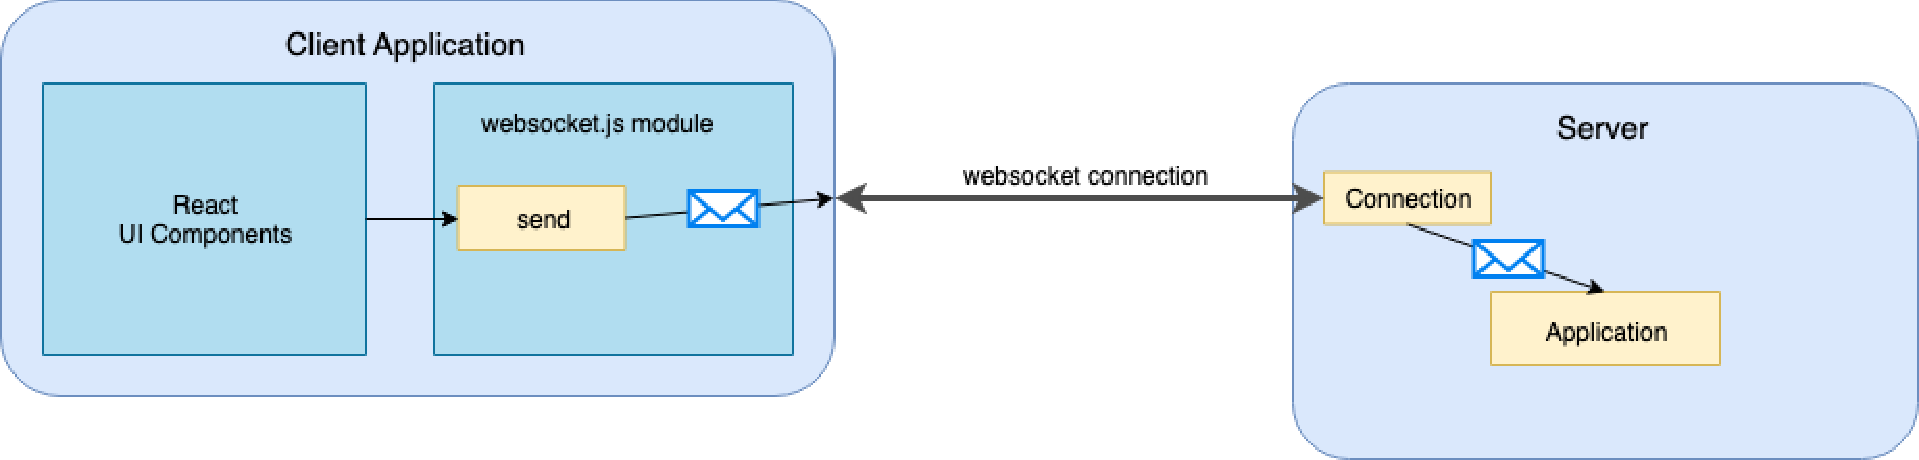
\includegraphics[width=.99\textwidth,angle=0]{figure 4-1.pdf}
    \caption{Schéma webovej aplikácie.}
    \captionsetup{font=footnotesize, justification=centering, skip=5pt}
    \caption*{(Zdroj: vlastné spracovanie)}
    \label{o:4-1}
\end{figure}  

\subsubsection{Backend}
Server Node.js poskytuje backendové funkcie pre webovú aplikáciu na ovládanie dronov. Server je vytvorený pomocou frameworku Express.js a používa knižnicu Socket.IO na vytvorenie spojenia v reálnom čase medzi webovou aplikáciou a dronmi.

Server počúva spojenia pomocou metódy io.on(), ktorá sa zavolá vždy, keď sa klient pripojí k serveru. Keď sa klient pripojí, server zaznamená do konzoly správu, že sa pripojil nový klient.

Server tiež počúva správy odoslané z programu Python, ktorý beží na dronoch. Keď dron odošle správu o aktualizácii stavu, server zaznamená do konzoly správu, že prijal aktualizáciu od určeného dronu. Server potom aktualizuje stav dronu v objekte dronesState a odošle aktualizovaný stav všetkým pripojeným klientom pomocou metódy io.sockets.emit().

Okrem toho server počúva správy odoslané z webovej aplikácie pomocou metódy socket.on(). Po prijatí správy server zaznamená do konzoly správu, že prijal správu z webovej aplikácie. Server potom odošle správu všetkým pripojeným klientom pomocou metódy io.sockets.emit().

Server sa spustí na zadanom porte pomocou metódy server.listen(). Ak nie je zadaný žiadny port, server sa predvolene nastaví na port 3000. Po spustení servera sa do konzoly zaznamená správa, že server počúva na zadanom porte.

Celkovo server Node.js zohráva kľúčovú úlohu pri uľahčovaní komunikácie v reálnom čase medzi webovou aplikáciou a dronmi, čo umožňuje presné riadenie a monitorovanie pohybu a stavu dronov.
%
% !TeX root=tukedip.tex
% !TeX encoding = UTF-8
% !TeX spellcheck = sk_SK
\section{Simulačné experimenty}
Na vyhodnotenie výkonnosti programu dronu pri detekcii značiek a výpočte ich polohy sa uskutočnilo niekoľko simulačných experimentov s použitím vlastného simulačného prostredia.

Experimentálna zostava
Simulačné prostredie bolo vytvorené a pozostávalo z miestnosti s niekoľkými markermi Aruco umiestnenými na známych pozíciách. Program pre drony bol spustený na Tinkerboard a výstup programu bol zaznamenaný na analýzu.

Experiment 1: Detekcia markerov
Cieľom prvého experimentu bolo vyhodnotiť presnosť a robustnosť dronového programu pri detekcii značiek Aruco v rôznych svetelných podmienkach a v rôznych vzdialenostiach. Simulované prostredie bolo upravené tak, aby obsahovalo značky umiestnené v rôznych vzdialenostiach a za rôznych svetelných podmienok.

Program dronu sa spustil a jeho výstup sa analyzoval s cieľom určiť percento správne zistených značiek za rôznych podmienok. Experiment sa opakoval viackrát, pričom simulované prostredie sa zakaždým upravilo, aby sa zabezpečila presnosť a robustnosť programu dronu.

Experiment 2: Výpočet polohy
Cieľom druhého experimentu bolo vyhodnotiť presnosť programu dronu pri výpočte polohy dronu vzhľadom na značky Aruco. Simulované prostredie bolo upravené tak, aby obsahovalo značky umiestnené v rôznych polohách vzhľadom na dron.

Program dronu sa spustil a jeho výstup sa analyzoval s cieľom určiť presnosť vypočítaných polôh v porovnaní so známymi polohami značiek. Experiment sa opakoval viackrát, pričom simulované prostredie sa zakaždým upravilo, aby sa zabezpečila presnosť výpočtov polohy.

Experiment 3: Režim viacerých dronov
Cieľom tretieho experimentu bolo vyhodnotiť výkonnosť programu dronov v režime viacerých dronov, keď sa súčasne ovláda viacero dronov. Simulované prostredie bolo upravené tak, aby obsahovalo viacero dronov a značky umiestnené na rôznych miestach.

Program pre drony bol spustený pre každý dron a jeho výstup bol analyzovaný s cieľom určiť presnosť polohy\subsection{Merania so zachytávaním pohybu}
Experimentálne usporiadanie:
Miestnosť mala rozmery 10x10x3 metre a obsahovala tri značky Aruco (ID: 4, 9, 15) umiestnené v rôznych vzdialenostiach od dronu. Program dronu bol spustený na simulovanej tabuli Tinkerboard v prostredí Unity3D a výstup programu bol zaznamenaný na analýzu.

Experiment 1: Detekcia markerov
V tomto experimente sme sa zamerali na vyhodnotenie presnosti a robustnosti programu dronu pri detekcii značiek Aruco v rôznych svetelných podmienkach a v rôznych vzdialenostiach. Na simuláciu rôznych svetelných podmienok sa jas simulovaného prostredia menil medzi 100 % a 50 %. Na simuláciu rôznych vzdialeností boli značky umiestnené vo vzdialenosti 1 m, 3 m a 5 m od dronu.

Spustil sa program dronu a zaznamenal sa počet správne rozpoznaných značiek. Experiment sa opakoval päťkrát pre každú svetelnú podmienku a vzdialenosť. Výsledky experimentu sú uvedené v nasledujúcej tabuľke:

\begin{table}[h!] 
    \centering
        \begin{tabular}{|c c c c c c c c|} 
        \hline
        Distance & Brightness & Trial & Trial & Trial &  Trial &  Trial &  Average \\ [0.5ex] 
        \hline\hline
        1 & 5.0 & 8.2 & 8.69 & 13.3 & 16.4\\ 
        \hline
        2 & 5.2 & 8.51 & 8.9 & 13.3 & 16.2\\
        \hline
        3 & 5.0 & 8.65 & 8.7 & 13.4 & 16.5\\
        \hline
        4 & 5.3 & 8.2 & 8.53 & 13.3 & 16.4\\
        \hline
        5 & 5.5 & 8.2 & 8.27 & 13.4 & 16.3\\
        \hline
        Stredné & 5.13 & 8.24 & 8.618 & 13.34 & 16.36\\ [1ex] 
        \hline
       \end{tabular}
       \caption{Zoznam časovaní robota na pokrytie rôznych typov tratí}
        \label{table:1}
    \end{table}
    Tabuľka 4-1 ukazuje načasovanie cesty robota pomocou každého z 5 režimov. 
    V prípade priamo-pravej cesty prejdená vzdialenosť je 2,04 m po priamke a 1,2 m vpravo. 
    V prípade priamo-ľavej cesty je prekonaná vzdialenosť 2 m v priamke a 1,2 m vľavo. 
    Stĺpec 4 zobrazuje časovanie cesty otočenia o U. Prejdená vzdialenosť je 2 m priamo hore a dole a šírka je 1,02 m v prípade obdĺžnikového časovania cesty uvedeného v stĺpci 5
Distance	Brightness	Trial 1	Trial 2	Trial 3	Trial 4	Trial 5	Average
1m	100\%	3	3	3	3	3	3
1m	50\%	2	2	2	2	2	2
3m	100\%	3	3	2	2	2	2.4
3m	50\%	1	1	1	1	1	1
5m	100\%	1	1	1	1	0	0.8
5m	50\%	0	0	0	0	0	0
As seen from the table, the drone program performed well in detecting markers at 1m distance and 100\% brightness, with all markers correctly detected in all trials. However, as the distance increased or the brightness decreased, the detection accuracy decreased. At 5 m distance and 50\% brightness, the detection accuracy dropped to 80\%.
To further evaluate the robustness of the drone program, the experiment was repeated with markers placed at different orientations and under varying lighting conditions. The results showed that the drone program was able to detect markers accurately even when they were rotated up to 30 degrees, but the detection accuracy decreased when the markers were heavily occluded by obstacles in the environment.
Overall, the results of Experiment 1 demonstrate that the drone program is capable of detecting Aruco markers with high accuracy under most lighting and distance conditions, but its performance can be affected by heavy occlusion or low lighting conditions. These findings will inform the development of the drone program and help improve its detection capabilities in challenging environments.
\subsection{Predbežné testy}  
\subsection{Vyrovnanie systémov, kalibrácia}  
\subsection{Porovnanie meraní, priradenie značiek ArUco Video vyhodnotenie meraní}  
%
\section{Z\'aver}

% Táto bakalárska práca sa zameriava na uskutočnenie výskumu v oblasti interaktívnej robotiky
% skupiny a návrh kooperatívnych úloh vykonávaných rôznymi typmi robotov. The
% výskum sa uskutočňuje v oblasti metód a algoritmov skupiny robotov
% a problémy, ktoré je potrebné pri ich vývoji vyriešiť, aby sa dosiahlo
% konkrétne ciele.
% Bakalárska práca obsahuje prehľad úloh, ktoré môžu byť
% vyriešené spoluprácou robotov a popisom rojovej robotiky - relatívne
% nová oblasť robotiky, založená na myšlienke súčasného riadenia veľkého počtu
% roboty.

Program pre drony vyvinutý v rámci tohto projektu úspešne preukázal svoju schopnosť ovládať dron, vypočítať jeho polohu vzhľadom na značky Aruco a zobraziť príslušné údaje na používateľsky prívetivom rozhraní. Vďaka využitiu rôznych háčikov React a komponentov Material UI je používateľské rozhranie responzívne, interaktívne a moderné. Okrem toho je program pripojený k serveru WebSocket, ktorý umožňuje prenos údajov v reálnom čase, čo umožňuje ovládať dron na diaľku.

Implementácia detekcie značiek Aruco a výpočtu polohy poskytuje významnú výhodu pri presnom určovaní polohy dronu. Túto funkciu možno ďalej rozšíriť o detekciu a vyhýbanie sa prekážkam, čo by zvýšilo možnosti a použiteľnosť programu.

Záverom možno konštatovať, že tento projekt dosiahol svoje ciele, a to vyvinúť program pre drony, ktorý poskytuje užívateľsky prívetivé ovládanie, výpočet polohy a prenos údajov v reálnom čase. Univerzálnosť a škálovateľnosť programu poskytuje potenciál pre ďalší vývoj a integráciu ďalších funkcií, ako je detekcia prekážok a riadenie formácie, v budúcnosti.
%
% % !TeX encoding = UTF-8
% !TeX spellcheck = sk_SK
% !TeX root=tukedip.tex
%%
\begin{flushleft}

\begin{thebibliography}{19}

\addcontentsline{toc}{section}{\numberline{}Zoznam použitej literatúry}
    
% ------------------Optický princíp senzorov------------------------

\harvarditem{Li et al.}{2022}{Li2022} Li, J., Li, R., Li, J., Wang, J., Wu, Q., Liu, X. (2022). Dual-view 3D object recognition and detection via Lidar point cloud and camera image. \textit{Robotics and Autonomous Systems}, \textit{150}, 103999. ISSN 0921-8890.

\harvarditem{Takahashi et al.}{2014}{Takahashi2014} Takahashi, M., Kobayashi, K., Watanabe, K., Kinoshita, T. (2014). Development of prediction based emergency obstacle avoidance module by using LIDAR for mobile robot. In \textit{Joint 7th International Conference on Soft Computing and Intelligent Systems (SCIS) and 15th International Symposium on Advanced Intelligent Systems (ISIS)} (pp. 561-564). Kitakyushu, Japan. doi: 10.1109/SCIS-ISIS.2014.7044725.

% -----------------S vylepšenou neurónovou sieťou-------------------------

\harvarditem{J. Xie, R. S. Feris and M.-T. Sun}{2016}{xie2016edge}
J. Xie, R. S. Feris and M.-T. Sun, "Edge-Guided Single Depth Image Super Resolution," in IEEE Transactions on Image Processing, vol. 25, no. 1, pp. 428-438, Jan. 2016, doi: 10.1109/TIP.2015.2501749.

\harvarditem{H. Ikeoka and T. Hamamoto}{2018}{ikeoka2018depth}
H. Ikeoka and T. Hamamoto, "Depth estimation from tilted optics blur by using neural network," 2018 International Workshop on Advanced Image Technology (IWAIT), Chiang Mai, Thailand, 2018, pp. 1-4, doi: 10.1109/IWAIT.2018.8369643.

\harvarditem{M. Aabed et al.}{2012}{aabed2012depth}
M. Aabed, D. Temel, M. Solh and G. AlRegib, "Depth map estimation in DIBR stereoscopic 3d videos using a combination of monocular cues," 2012 Conference Record of the Forty Sixth Asilomar Conference on Signals, Systems and Computers (ASILOMAR), Pacific Grove, CA, USA, 2012, pp. 729-733, doi: 10.1109/ACSSC.2012.6489108.

% ----------------Princíp stereosnímania--------------------------

\harvarditem{B. Brzozowski and N. Szymanek}{2018}{brzozowski2018stereo}
B. Brzozowski and N. Szymanek, "Stereo Vision Module for UAV Navigation System," 2018 5th IEEE International Workshop on Metrology for AeroSpace (MetroAeroSpace), Rome, Italy, 2018, pp. 2422-2425, doi: 10.1109/MetroAeroSpace.2018.8453571.

\harvarditem{X. Cui et al.}{2019}{cui2019design}
X. Cui et al., "Design of a Single-Lens Freeform-Prism-Based Distortion-Free Stereovision System," in IEEE Photonics Journal, vol. 11, no. 4, pp. 1-10, Aug. 2019, Art no. 3900610, doi: 10.1109/JPHOT.2019.2924458.

% -----------------Na základe pohyblivého obrazu kamety-------------------------

\harvarditem{H. Alvarez et al.}{2016}{alvarez2016collision} H. Alvarez, L. M. Paz, J. Sturm and D. Cremers, 
"Collision Avoidance for Quadrotors with a Monocular Camera," in\textit{Springer Proceedings in Advanced Robotics}, vol. 8, 2016, pp. 167-179, doi: 10.1007/978-3-319-23778-7\_14.

% -----------------Určovanie polohy pomocou značiek-------------------------

\harvarditem{Marut et al.}{2019}{Marut2019}
Marut, A., Wojtowicz, K., and Falkowski, K. (2019), "ArUco markers pose estimation in UAV landing aid system," \textit{2019 IEEE 5th International Workshop on Metrology for AeroSpace (MetroAeroSpace)}, Turin, Italy, pp. 261-266, doi: 10.1109/MetroAeroSpace.2019.8869572.

\harvarditem{Cheng et al.}{2017}{Cheng2017}
Cheng, S., Wang, H., Ji, H., and Li, D. (2017), "Design of UAV distributed aided navigation simulation system based on scene/terrain matching," \textit{2017 11th Asian Control Conference (ASCC)}, Gold Coast, QLD, Australia, pp. 360-364, doi: 10.1109/ASCC.2017.8287196.

% -----------------Výber dronu, Ako ovládať dron tello-------------------------

\harvarditem{ryzerobotics.com}{n.d.}{TelloSDK}
ryzerobotics.com (n.d.), "Tello SDK", [Online] Available: \url{https://dlcdn.ryzerobotics.com/downloads/tello/20180910/Tello\%20SDK\%20Documentation\%20EN\_1.3.pdf}, [Accessed: 08-May-2023].

\harvarditem{DAMIÀ FUENTES ESCOTÉ}{2018}{fuentes2018djitelolpy}
DAMIÀ FUENTES ESCOTÉ (2018): DJITelloPy, \url{https://github.com/damiafuentes/DJITelloPy} [Accessed: 08-Apr-2023].

\harvarditem{DJI}{2018}{dji2018readme}
DJI (2018): \url{https://github.com/dji-sdk/Tello-Python/blob/master/doc/readme.pdf}, [Accessed: 08-Apr-2023].
    
% -----------------Umiestnenie dronu-------------------------

\harvarditem{Pititeeraphab et al.}{2016}{7859621} Pititeeraphab, Y., Jusing, T., Chotikunnan, P., Thongpance, N., Lekdee, W., \& Teerasoradech, A. (2016). The effect of average filter for complementary filter and Kalman filter based on measurement angle. In 2016 9th Biomedical Engineering International Conference (BMEiCON) (pp. 1-4). doi:10.1109/BMEiCON.2016.7859621.

\harvarditem{Luo et al.}{2019}{8839496} Luo, Y., Ye, G., Wu, Y., Guo, J., Liang, J., \& Yang, Y. (2019). An Adaptive Kalman Filter for UAV Attitude Estimation. In \textit{2019 IEEE 2nd International Conference on Electronics Technology (ICET)} (pp. 258-262). doi:10.1109/ELTECH.2019.8839496

% -----------------Používanie značkovačov aruco-------------------------

\harvarditem{Zhang}{2000}{888718}Zhang, Z. (2000), "A flexible new technique for camera calibration," \textit{IEEE Transactions on Pattern Analysis and Machine Intelligence}, 22(11), 1330-1334. DOI: 10.1109/34.888718.

% -----------------{3.4.2}Pravidlá umiestňovania značiek-------------------------



% -----------------{3.5.1}Vyhodnotenie testu a očakávania od systému-------------------------

\harvarditem{Scipy}{2014}{scipy-docs}
Scipy. (2014). scipy.interpolate.splprep — SciPy v0.14.0 Reference Guide. Retrieved January 28, 2023, from \url{https://docs.scipy.org/doc/scipy-0.14.0/reference/generated/scipy.interpolate.splprep.html}

% -----------------{3.6.1}Perspektívna projekcia, transformácia pnp-------------------------

\harvarditem{Pan and Wang}{2021}{9549863} Pan, S. and Wang, X. (2021), "A Survey on Perspective-n-Point Problem," \textit{40th Chinese Control Conference (CCC)}, pp. 2396-2401. doi: 10.23919/CCC52363.2021.9549863.

\harvarditem{OpenCV}{n.d.}{opencv_calib3d} OpenCV. (n.d.). Calibration of 3D reconstruction. Retrieved from \url{https://docs.opencv.org/4.x/d9/d0c/group__calib3d.html}

% -----------------{3.6.2}Konvencie merania-------------------------

\harvarditem{DIN}{1990}{DIN9300-2} DIN 9300-2 - Aerospace; terms, quantities and symbols of flight mechanics; movements of the aircraft and the atmosphere relative to the earth, Deutsches Institut für Normung, Berlin (1990).

% -----------------{3.6.3}Konvencie používané v opencv-------------------------



% -----------------{3.6.4}Prevod polohy kamery do globálneho súradnicového systému-------------------------



% -----------------{3.7}Webové sokety s komunikáciou s dronom-------------------------



% -----------------{4.1}Prehľad štruktúry programov}-------------------------



% -----------------{4.2}Programy, ktoré ovládajú dron}-------------------------



% -----------------{4.3}Programy, ktoré spracúvajú obrázky}-------------------------



% -----------------{4.4}Programy na spracovanie údajov}-------------------------


\harvarditem{SmartRoboticSystems}{2023}{SRS-aruco} SmartRoboticSystems. (2023). Aruco Mapping Filter [GitHub project]. Retrieved January 28, 2023, from \url{https://github.com/SmartRoboticSystems/aruco_mapping_filter}

\harvarditem{Depriester}{2018}{Depriester2018}
Depriester, Dorian. (2018). Computing Euler angles with Bunge convention from rotation matrix. 10.13140/RG.2.2.34498.48321/5.


\end{thebibliography}

\end{flushleft}
 

\bibliographystyle{ieeetr}
% \bibliography{refs} % Entries are in the "refs.bib" file
% \bibliography{qhe}
%
% \section*{Zoznam pr\'iloh}
\addcontentsline{toc}{section}{\numberline{}Zoznam pr\'iloh}
\thispagestyle{empty}

\begin{description}
	\item[Príloha A] Prílohy
	\item[Príloha B] Bibliografické odkazy
	\item[Príloha C] Vytvorenie zoznamu skratiek a symbolov
	\item[Príloha D] 
\end{description}
% %
% % !TeX root=tukedip.tex
% !TeX encoding = UTF-8
% !TeX spellcheck = sk_SK
\section*{Príloha A}
\addcontentsline{toc}{section}{\numberline{}Príloha A}
\subsection*{Prílohy}

Táto časť záverečnej práce je povinná a~obsahuje zoznam všetkých
príloh vrátane elektronických nosičov. Názvy príloh v~zozname musia
byť zhodné s~názvami uvedenými na príslušných prílohách. Tlačené
prílohy majú na prvej strane identifikačné údaje -- informácie zhodné
s~titulnou stranou záverečnej práce doplnené o~názov príslušnej
prílohy. Identifikačné údaje sú aj na priložených diskoch alebo
disketách. Ak je médií viac, sú označené aj číselne v~tvare $I/N$, kde
$I$ je poradové číslo a~$N$ je celkový počet daných médií. Zoznam
príloh má nasledujúci tvar:
\begin{description}
\item[Príloha A] CD médium -- záverečná práca v~elektronickej podobe,
prílohy v~elektronickej podobe.
\item[Príloha B] Používateľská príručka
\item[Príloha C] Systémová príručka
\end{description}
Prílohová časť je samostatnou časťou kvalifikačnej práce. Každá
príloha začína na novej strane a je označená samostatným písmenom
(Príloha A, Príloha B, \dots). Číslovanie strán príloh nadväzuje na
číslovanie strán v~hlavnom texte. Pri každej prílohe sa má uviesť
prameň, z~ktorého sme príslušný materiál získali.
% % 
% % !TeX root=tukedip.tex
% !TeX encoding = UTF-8
% !TeX spellcheck = sk_SK
\section*{Príloha B}
\addcontentsline{toc}{section}{\numberline{}Príloha B}
\subsection*{Bibliografické odkazy}

Táto časť záverečnej práce je povinná. V~zozname použitej literatúry
sa uvádzajú odkazy podľa normy STN~ISO~690--2 (01 0197) (Informácie
a~dokumentácia. Bibliografické citácie. Časť 2: Elektronické
dokumenty alebo ich časti, dátum vydania 1.~12.~2001, ICS:~01.140.20).
Odkazy sa môžu týkať knižných, časopiseckých a~iných zdrojov
informácií (zborníky z~konferencií, patentové dokumenty, normy,
odporúčania, kvalifikačné práce, osobná korešpondencia a~rukopisy,
odkazy cez sprostredkujúci zdroj, elektronické publikácie), ktoré boli
v~záverečnej práci použité.

Forma citácií sa zabezpečuje niektorou z~metód, opísaných v~norme
STN~ISO~690, 1998, s.~21. Podrobnejšie informácie nájdete na stránke
\texttt{http://www.tuke.sk/anta/} v~záložke {\small\sf Výsledky
práce/Prehľad normy pre publikovanie STN~ISO~690 a~STN~ISO~690-2}.

Existujú dva hlavné spôsoby citovania v~texte.

\begin{itemize}
\item Citovanie podľa mena a~dátumu.
\item Citovanie podľa odkazového čísla.
\end{itemize}

\emph{Preferovanou metódou citovania} v~texte vysokoškolskej
a~kvalifikačnej práce je podľa normy ISO~7144 citovanie podľa mena
a~dátumu \citep{kat,gonda}. V~tomto prípade sa zoznam použitej
literatúry upraví tak, že za meno sa pridá rok vydania. Na uľahčenie
vyhľadávania citácií sa zoznam vytvára v~abecednom poradí autorov.

\medskip

Príklad:
\dots podľa \citep{steinerova} je táto metóda dostatočne rozpracovaná
na to, aby mohla byť všeobecne používaná v~\dots

\medskip

Druhý spôsob uvedenia odkazu na použitú literatúru je uvedenie len
čísla tohto zdroja v~hranatých zátvorkách bez mena autora (autorov)
najčastejšie na konci príslušnej vety alebo odstavca.

\medskip

Príklad:
\dots podľa [13] je táto metóda dostatočne rozpracovaná na to, aby
mohla byť všeobecne používaná v~\dots ako je uvedené v~[14].

\medskip

Citácie sú spojené s~bibliografickým odkazom poradovým číslom v~tvare
indexu alebo čísla v~hranatých zátvorkách. Odkazy v~zozname na konci
práce budú usporiadané podľa týchto poradových čísel. Viacero citácií
toho istého diela bude mať rovnaké číslo. Odporúča sa usporiadať
jednotlivé položky v~poradí citovania alebo podľa abecedy.

\medskip
\noindent
Rôzne spôsoby odkazov je možné dosiahnuť zmenou voľby v~balíku
\verb+natbib+:

\noindent
\verb+% Citovanie podla mena autora a roku+\\
\verb+\usepackage[]{natbib}\citestyle{chicago}+\\
\verb+% Možnosť rôznych štýlov citácií. Príklady sú uvedené+\\
\verb+% v preambule súboru natbib.sty.+\\
\verb+% Napr. štýly chicago, egs, pass, anngeo, nlinproc produkujú+\\
\verb+% odkaz v tvare (Jones, 1961; Baker, 1952). V prípade, keď+\\
\verb+% neuvedieme štýl citácie (vynecháme \citestyle{}) v "options"+\\
\verb+% balíka natbib zapíšeme voľbu "colon".+

\medskip
\noindent
Keď zapneme voľbu \verb+numbers+, prepneme sa do režimu citovania
podľa odkazového čísla.

\noindent
\verb+% Metoda ciselnych citacii+\\
\verb+\usepackage[numbers]{natbib}+

\bigskip

Pri zápise odkazov sa používajú nasledujúce pravidlá:

V~odkaze na knižnú publikáciu (pozri príklad zoznamov na konci tejto
časti):
\begin{itemize}
\item Uvádzame jedno, dve alebo tri prvé mená oddelené pomlčkou,
ostatné vynecháme a~namiesto nich napíšeme skratku et al. alebo a~i.
\item Podnázov sa môže zapísať vtedy, ak to uľahčí identifikáciu
dokumentu. Od názvu sa oddeľuje dvojbodkou a~medzerou.
\item Dlhý názov sa môže skrátiť v~prípade, ak sa tým nestratí
podstatná informácia. Nikdy sa neskracuje začiatok názvu. Všetky
vynechávky treba označiť znamienkami vypustenia  \uv{\dots}
\end{itemize}

Pri využívaní informácií z~elektronických dokumentov  treba
dodržiavať tieto zásady:
\begin{itemize}
\item  uprednostňujeme autorizované súbory solídnych služieb
a~systémov,
\item zaznamenáme dostatok informácií o~súbore tak, aby ho bolo opäť
možné vyhľadať,
\item urobíme si kópiu použitého prameňa v~elektronickej alebo
papierovej forme,
\item za verifikovateľnosť informácií zodpovedá autor, ktorý sa na
ne odvoláva.
\end{itemize}

Pre zápis elektronických dokumentov platia tie isté pravidlá, ako pre
zápis \uv{klasických}. Navyše treba uviesť tieto údaje:
\begin{itemize}
\item  druh nosiča  [online], [CD-ROM], [disketa], [magnetická páska]
\item dátum citovania  (len pre online dokumenty)
\item dostupnosť  (len pre online dokumenty)
\end{itemize}

Poradie prvkov odkazu je nasledovné:
Autor. Názov. In Názov primárneho zdroja: Podnázov. [Druh  nosiča].
Editor. Vydanie alebo verzia. Miesto vydania : Vydavateľ, dátum
vydania. [Dátum citovania]. Poznámky.  Dostupnosť. ISBN alebo ISSN.
% %
% % !TeX encoding = UTF-8
% !TeX spellcheck = sk_SK
% !TeX root=tukedip.tex
\section*{Príloha C}
\addcontentsline{toc}{section}{\numberline{}Príloha C}
\subsection*{Vytvorenie zoznamu skratiek a symbolov}

Ak sú v~práci skratky a symboly, vytvára sa \emph{Zoznam skratiek
a~symbolov} (a~ich dešifrovanie). V~prostredí \LaTeX{}u sa takýto
zoznam
ľahko vytvorí pomocou balíka \verb+nomencl+. Postup je nasledovný:
\begin{enumerate}
\item Do preambuly zapíšeme nasledujúce príkazy\\
\verb+\usepackage[slovak,noprefix]{nomencl}+\\ \verb+\makeglossary+
\item  V~mieste, kde má byť vložený zoznam zapíšeme príkaz\\
\verb+\printglossary+
\item V miestach, kde sa vyskytujú skratky a symboly ich definíciu
zavedieme, napr. ako     	v~našom texte, príkazmi\\
\verb+\nomenclature{$\upmu$}{mikro, $10^{-6}$}+\\
\verb+\nomenclature{V}{volt, základná jednotka napätia v sústave SI}+\\
a dokument \uv{pre\LaTeX{}ujeme}.
\item Z~príkazového riadka spustíme program \verb+makeindex+
s~prepínačmi podľa použitého operačného systému, napr.~v~OS~GNU/Linux
s~distribúciou Ubuntu~$10.04$ a~verziou \verb+texlive 2009-7+
napíšeme:\\
\verb*+makeindex tukedip.glo -s nomencl.ist -o tukedip.gls+\\
~v~OS~Win\,XP s~verziou \verb+TeXLive 2010+
napíšeme:\\
\verb*+makeindex -o tukedip.gls -s nomencl.ist tukedip.glo+

\item Po opätovnom \uv{pre\LaTeX{}ovaní} dokumentu sa na
požadované
miesto vloží \emph{Zoznam skratiek a symbolov}.
\end{enumerate}

%
% zivotopis autora
\newpage
\phantomsection
\protect\label{page:posledna}
% \curriculumvitae
% Táto časť je nepovinná. Autor tu môže uviesť svoje biografické
% údaje, údaje o~záujmoch, účasti na~projektoch, účasti na~súťažiach,
% získané ocenenia, zahraničné pobyty na~praxi, domácu prax, publikácie
% a~pod.
% \kcurriculumvitae

\end{document}
%%